% Compile directly with pdfLaTeX and BibTeX. For manuscript inclusion,
% load natbib, longtable, graphicx, tikz, booktabs and hyperref, then
% define \INERTmanuscript before % Compile directly with pdfLaTeX and BibTeX. For manuscript inclusion,
% load natbib, longtable, graphicx, tikz, booktabs and hyperref, then
% define \INERTmanuscript before % Compile directly with pdfLaTeX and BibTeX. For manuscript inclusion,
% load natbib, longtable, graphicx, tikz, booktabs and hyperref, then
% define \INERTmanuscript before % Compile directly with pdfLaTeX and BibTeX. For manuscript inclusion,
% load natbib, longtable, graphicx, tikz, booktabs and hyperref, then
% define \INERTmanuscript before \input{injection_channel_taxonomy}.
\ifdefined\INERTmanuscript\else
\documentclass[11pt]{article}
\usepackage[margin=23mm]{geometry}
\usepackage[numbers,sort&compress]{natbib}
\usepackage{longtable,graphicx,tikz,booktabs,xurl}
\usepackage[colorlinks=true,citecolor=teal,urlcolor=teal,linkcolor=teal]{hyperref}
\setlength{\parindent}{0pt}\setlength{\parskip}{5pt}
\begin{document}
\fi
\section{A Taxonomy of Injection Channels in Agent Collaboration}\label{sec:taxonomy}

A reader agent may be authorized to summarize a document, a coordinator to assign work, and a publisher to release a report. The document can legitimately influence the report's contents. It becomes a security concern if text derived from that document can also determine who receives the report or whether it is released. The distinction turns on the authority of the receiving decision. Even a correctly authenticated summary can carry information whose original author had no authority over that decision~\citep{greshake2023indirect,triedman2025mas,debenedetti2025camel}.

\subsection{Unit of analysis and classification rule}

We define an \emph{injection channel} as a path by which externally influenced content reaches a component that can interpret it as an instruction or use it to make a protected decision. For each observed handoff we record the \emph{source} that supplied the content, the \emph{carrier} that conveyed it, the \emph{consumer} that interpreted it, and the \emph{decision} that the workflow authorizes that consumer to make. We also record the attacker's assumed access, how long the content remains available, and what the execution trace actually establishes. An origin such as a compromised worker describes who can act. An outcome such as disclosure describes what happened. Either can occur across several channels.

Table~\ref{tab:channels-inert} classifies each handoff by the interface through which the receiving component obtains the content. A run can cross several interfaces. For example, a document read from an issue tracker, summarized by a worker, and retained for a later session crosses the external-content, peer-message, and shared-state channels in sequence. If the summary is later read to choose a recipient, that last use is a protected decision. Counting each handoff retains both the original source and the later point at which the application grants the value authority. This decomposition complements existing taxonomies of entry points and multi-agent attack paths~\citep{Mitra2026WhereREC,Yang2026SoKWSJ,Paul2026BeyondSIE}.


\begin{longtable}{@{}p{.16\linewidth}@{\hspace{.02\linewidth}}p{.25\linewidth}@{\hspace{.02\linewidth}}p{.27\linewidth}@{\hspace{.02\linewidth}}p{.25\linewidth}@{}}
\caption{Injection channels classified by receiving interface. The final column gives an example of a policy obligation a developer can express and check.}\label{tab:channels-inert}\\
\hline\textbf{Channel} & \textbf{Source and carrier} & \textbf{Consumer and decision} & \textbf{Example obligation}\\\hline\endfirsthead
\hline\textbf{Channel} & \textbf{Source and carrier} & \textbf{Consumer and decision} & \textbf{Example obligation}\\\hline\endhead
User request & A caller supplies a task, clarification, or conversational reply. & An intake agent interprets the request and chooses its scope. & Bind each request to its principal, task, and permitted operations.\\[3pt]
External content & An external author supplies a document, issue, email, or image that an agent retrieves. & A reader extracts facts that may later influence other agents. & Retrieved content may populate report text. Release approval requires an independent authorized source.\\[3pt]
Tool response & A service returns data or diagnostic text from a permitted tool call. & A worker interprets the result, or a coordinator uses reported status to select a next step. & Bind the response to its invocation. Validate control-relevant status separately from free text.\\[3pt]
Peer message & A worker, reviewer, or intermediary supplies a message, summary, or proposed value. & A peer incorporates the value into its reasoning or output. & Check sender, role, request, and permitted dependencies of the receiving field.\\[3pt]
Coordination signal & An agent reports completion, failure, a review verdict, or a delegation request. & An orchestrator chooses a transition, successor, retry, or release. & Accept only authorized transitions for the current workflow state and request.\\[3pt]
Shared state & A prior task, peer, or external writer contributes a memory, blackboard item, or knowledge-base record. & A later retrieval introduces the value into a new decision context. & Scope reads by principal and task, and retain the provenance of retrieved values.\\[3pt]
Discovery metadata & A provider publishes an agent description, skill declaration, or tool record. & A planner or registry resolves a name, selects a provider, or grants a capability. & Bind the approved identity and metadata version to the invocation.\\\hline
\end{longtable}

\subsection{Propagation, authority, and observable effects}

A peer message and a coordination signal can share the same transport. The distinction is the recipient's use of the field. A worker's narrative about a failed read is a peer message. A failure status that the controller accepts as authority to change the next step is a coordination signal. Likewise, an email returned by a tool has an external author and a tool-response envelope. Recording both avoids attributing the authority of the tool service to the author of the email. Registration-time influence occurs earlier still, when the planner first learns what a participant claims it can do~\citep{Yu2026MisleadingTPO}.

Three properties cut across the channels. First, influence can survive a transformation. A summary can preserve a request's meaning after its wording changes, and independently innocuous fragments can acquire a different meaning when agents combine them~\citep{lee2024promptinfection,arif2026conjunctive}. Second, the influence can outlive the interaction. Work on poisoned retrieval and cross-user context motivates recording which task wrote a value and which task subsequently read it~\citep{Chen2024AgentPoisonRLBS,Patlan2025CrossUserPUAK}. Third, authority can change along the path. A read-only worker can influence a peer with publishing privileges. The roles, topology, and memory visible to each agent therefore matter even when the agents use the same underlying model~\citep{hagag2026architecture,naik2026omnileak}.

For each boundary we distinguish \emph{exposure}, when a consumer receives the value, \emph{proposal}, when a component requests an action, \emph{acceptance}, when a controller authorizes it, and \emph{effect}, when there is evidence of a disclosure or state change. A denied proposal and a successful disclosure warrant different verdicts. A record that an executor accepted a request establishes acceptance. Establishing delivery to an external recipient may also require a service receipt or observable state change. A malicious participant that directly misuses an allowed tool is an important comparison case: attribution to injection requires evidence of an influencing input~\citep{kavathekar2025tamas}.

\subsection{Evidence from the studies}

Table~\ref{tab:channel-evidence} decomposes the studies that anchor the channel definitions. Its last column gives our interpretation of the evidence for a workflow designer. Benchmarks supply defined scenarios, architecture studies vary system choices, and defense papers identify potential enforcement points. These forms of evidence support different conclusions. In particular, a defense evaluated on tool-response injection does not by itself establish protection against a compromised participant or a value retrieved by another user.

\begin{longtable}{@{}p{.19\linewidth}@{\hspace{.02\linewidth}}p{.22\linewidth}@{\hspace{.02\linewidth}}p{.24\linewidth}@{\hspace{.02\linewidth}}p{.28\linewidth}@{}}
\caption{Study-level evidence. The study design appears beneath each citation. Carrier, receiving decision, and implication are coded separately.}\label{tab:channel-evidence}\\
\hline\textbf{Study} & \textbf{Source and carrier} & \textbf{Consumer or decision} & \textbf{Implication for testing}\\\hline\endfirsthead
\hline\textbf{Study} & \textbf{Source and carrier} & \textbf{Consumer or decision} & \textbf{Implication for testing}\\\hline\endhead
Indirect injection~\citep{greshake2023indirect}\par{\footnotesize\itshape Application case studies} & External author, retrieved content & Application reads data for a legitimate task & The document author and the caller can have different authority.\\[3pt]
InjecAgent~\citep{zhan2024injecagent}\par{\footnotesize\itshape Tool-use benchmark} & Tool service, returned content & Agent considers a subsequent tool action & A permitted read can expose an agent to unauthorized instructions.\\[3pt]
Email-agent detection~\citep{Hashmi2026PromptIDBR}\par{\footnotesize\itshape Email-agent detection study} & Email author, message content & Email agent processes a sequence of events & The email is an entry point; later decisions determine the effect.\\[3pt]
Prompt Infection~\citep{lee2024promptinfection}\par{\footnotesize\itshape Propagation experiments} & Peer, generated message & Other agents consume and reproduce instructions & Record each receiving agent, including peers that only relay content.\\[3pt]
Agent-in-the-Middle~\citep{he2025aitm}\par{\footnotesize\itshape Communication threat model} & Intermediary, inter-agent message & Recipient reads a modified message & Message integrity and sender authorization require separate checks.\\[3pt]
Conjunctive prompts~\citep{arif2026conjunctive}\par{\footnotesize\itshape Composition experiments} & Multiple inputs, routed segments & A downstream component combines context & A component-level verdict can miss a property of the combined input.\\[3pt]
Control-flow hijacking~\citep{triedman2025mas}\par{\footnotesize\itshape Orchestration experiments} & External content, reported status & Orchestrator selects a privileged next step & Record the transition and its authorizing evidence.\\[3pt]
ControlValve~\citep{jha2025controlvalve}\par{\footnotesize\itshape Control-flow defense} & Coordinator, invocation request & Controller checks graph and contextual rules & An allowed edge and an allowed invocation context are distinct obligations.\\[3pt]
Registration-time injection~\citep{Yu2026MisleadingTPO}\par{\footnotesize\itshape Planner-registration study} & Provider, worker description & Central planner chooses a worker & Provider-supplied claims can influence delegation before task execution.\\[3pt]
Tool squatting~\citep{Narajala2025SecuringGMAU}\par{\footnotesize\itshape Registry-based defense} & Provider, tool registration & Registry or planner resolves tool identity & Test identity resolution separately from authorization of arguments.\\[3pt]
AgentPoison~\citep{Chen2024AgentPoisonRLBS}\par{\footnotesize\itshape Retrieval-poisoning study} & External writer, persistent memory & Retriever brings a stored record into context & Record write provenance as well as the later retrieval.\\[3pt]
Cross-user poisoning~\citep{Patlan2025CrossUserPUAK}\par{\footnotesize\itshape Cross-user threat model} & Different principal, shared history & Shared agent acts in another task context & The identity of the current user is part of the authorization decision.\\[3pt]
Terrarium~\citep{Nakamura2025TerrariumRTAR}\par{\footnotesize\itshape Blackboard research framework} & Participants, shared blackboard & Agents read and contribute shared state & A shared-store model makes reads and writes explicit.\\[3pt]
OMNI-LEAK~\citep{naik2026omnileak}\par{\footnotesize\itshape Confidentiality study} & Multiple agents, cross-role data & Sensitive data reaches an external communication capability & Audit the destination and the provenance of released data.\\[3pt]
Architecture Matters~\citep{hagag2026architecture}\par{\footnotesize\itshape Architecture comparison} & Role, topology, memory visibility & Architecture changes opportunities for exposure and action & Compare stage-specific outcomes across architectures.\\[3pt]
TAMAS~\citep{kavathekar2025tamas}\par{\footnotesize\itshape Multi-agent benchmark} & External input or compromised participant & Agents interact across benchmark configurations & Stratify by attacker placement and retain benign utility.\\[3pt]
ACIArena~\citep{An2026ACIArenaTUH}\par{\footnotesize\itshape Cascading-injection benchmark} & External inputs, agent profiles, peer messages & Benchmark tracks instruction hijacking, task disruption, and disclosure & Its 1,356 cases across six implementations separate the entry surface from the attack objective.\\[3pt]
Judgment boundary~\citep{Mitra2026WhereREC}\par{\footnotesize\itshape Layered policy evaluation} & Multiple entry points, policy-relevant inputs & Layered checks and judgments mediate decisions & Identify which verdicts follow from explicit rules and which require interpretation.\\[3pt]
CaMeL~\citep{debenedetti2025camel}\par{\footnotesize\itshape Information-flow defense} & Untrusted data, tool arguments & Program interpreter checks authorized flows & A fixed plan still needs a policy for values reaching tool calls.\\[3pt]
DRIFT~\citep{li2025drift}\par{\footnotesize\itshape Runtime defense} & Tool interactions, memory stream & Validator and isolator mediate evolving context & A change in permissions and a persistent record require different checks.\\[3pt]
Robotic systems~\citep{Nagaraja2026WhenPCBF}\par{\footnotesize\itshape Robotic task evaluation} & Agent inputs, multi-agent decisions & Robotic task execution can exhibit unintended behavior & Define the effect in the application's observable state.\\[3pt]
\hline\end{longtable}

\subsection{From channel categories to model-based test obligations}

For each modeled channel, a developer can identify a permitted use, a protected decision, and an observable event that distinguishes them. In the report workflow, a positive test checks that document-derived text may enter the summary. A companion test checks whether a value with that same provenance can become release approval. A third checks whether the authorized reviewer can still approve the current report. The three observations distinguish successful task execution, enforcement of the source restriction, and an overly restrictive policy that suppresses useful work.

The structural obligations concern the identity of the sender, the current request, the selected transition, and the tool bound to the invocation. Information-flow obligations concern the dependencies of the accepted value. A permitted author can still submit a value derived from a disallowed source. Conversely, an agent can submit a well-typed but factually wrong summary within its authority. INERT checks the modeled permissions and dependencies; factual correctness requires an appropriate content oracle. Coverage is relative to the declared model, and an observed run supplies evidence only about the events visible to its oracle. This interpretation connects scenario-based evaluation and structural workflow coverage to the generation criteria in the test-generation section~\citep{debenedetti2024agentdojo,kahani2026structural}.


Table~\ref{tab:channel-oracles} gives paired observations for the seven interfaces. The examples specify what an evaluator would need to observe. They are proposed test obligations derived from the taxonomy.

\begin{longtable}{@{}p{.16\linewidth}@{\hspace{.02\linewidth}}p{.25\linewidth}@{\hspace{.02\linewidth}}p{.25\linewidth}@{\hspace{.02\linewidth}}p{.27\linewidth}@{}}
\caption{Channel-specific evidence for authority, benign utility, and policy violations. Each row describes one possible policy and its oracle.}\label{tab:channel-oracles}\\
\toprule\textbf{Interface} & \textbf{Binding to record} & \textbf{Benign witness} & \textbf{Violation witness}\\\midrule\endfirsthead
\toprule\textbf{Interface} & \textbf{Binding to record} & \textbf{Benign witness} & \textbf{Violation witness}\\\midrule\endhead
User request & Caller identity, task owner, active request. & A caller revises a task that they own. & A revision is committed to another principal's task without delegated authority.\\[4pt]
External content & Document identity, derived fields, release policy. & The report includes facts from the retrieved document. & Release approval is accepted from a value derived solely from document text.\\[4pt]
Tool response & Call identifier, expected responder, status field. & A result updates the field requested by the pending call. & A result for an earlier call is accepted as the current call's completion.\\[4pt]
Peer message & Authorized author, destination field, request version. & The assigned reviewer supplies a verdict for the current revision. & A different peer or a stale review fills the protected verdict field.\\[4pt]
Coordination signal & Current workflow state, transition, role required to authorize it. & A valid review advances the current report to release. & A release transition occurs without an accepted review for that report.\\[4pt]
Shared state & Record writer, owner, visibility, task of subsequent read. & A worker retrieves its own task's permitted notes. & A private record from another task appears in the worker's delivered context.\\[4pt]
Discovery metadata & Approved provider identity, descriptor version, resolved executable. & The dispatcher invokes the provider and version approved for the task. & The dispatcher binds the invocation to a provider outside the approved set.\\[4pt]
\bottomrule\end{longtable}

\subsection{Research branches represented in the corpus}

Figure~\ref{fig:inert-corpus-tree} classifies the indexed literature by primary research focus. For example, a study of how one agent's message influences another follows the path from threats and propagation to threat mechanisms and then to peer influence and composition. Each study appears at one leaf.

\begin{figure}[p]
\centering
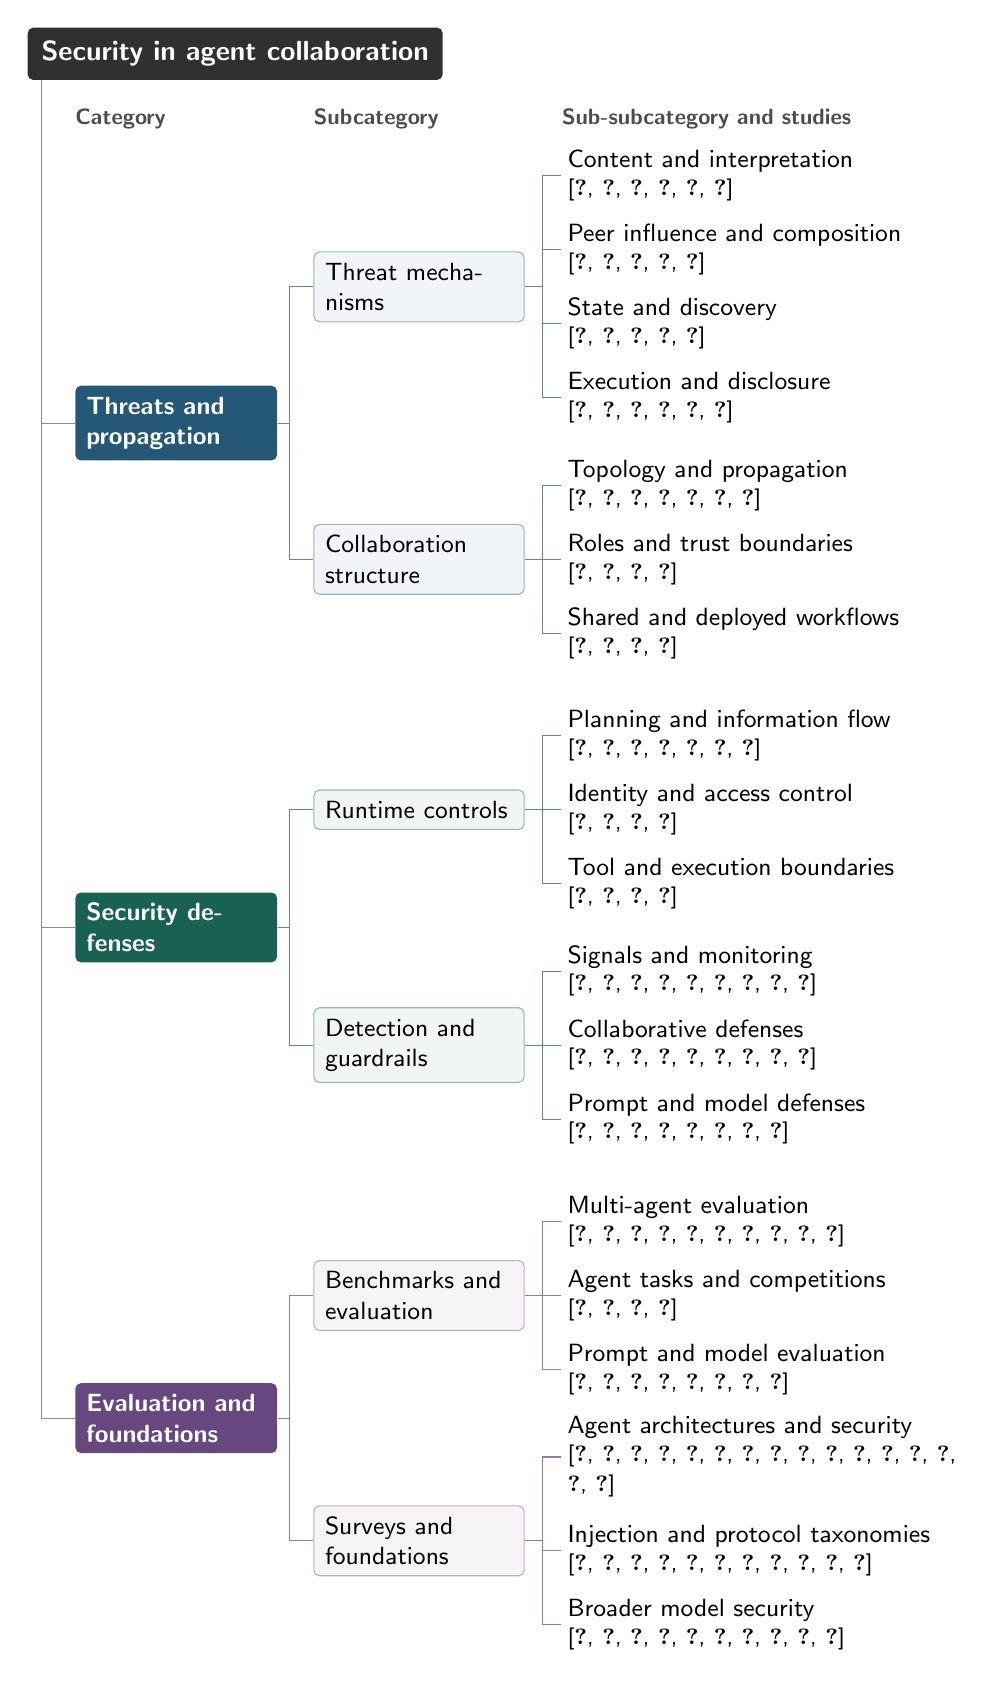
\begin{tikzpicture}[x=.01\linewidth,y=1cm,
  root/.style={anchor=west,rounded corners=2pt,fill=black!81,text=white,inner sep=5pt,font=\sffamily\bfseries},
  cat/.style={anchor=west,align=left,text width=.188\linewidth,inner sep=4pt,rounded corners=2pt,font=\sffamily\small\bfseries},
  sub/.style={anchor=west,align=left,text width=.197\linewidth,inner sep=4pt,rounded corners=2pt,font=\sffamily\small},
  leaf/.style={anchor=west,align=left,text width=.423\linewidth,inner sep=2pt,font=\sffamily\small},
  level/.style={anchor=west,font=\sffamily\footnotesize\bfseries,text=black!70,inner sep=0pt}]
\node[root] (root) at (0,1.42) {Security in agent collaboration};
\node[level] at (5,.59) {Category};
\node[level] at (30,.59) {Subcategory};
\node[level] at (56,.59) {Sub-subcategory and studies};
\definecolor{tier0}{HTML}{245876}
\definecolor{tier1}{HTML}{196253}
\definecolor{tier2}{HTML}{674780}
\coordinate (origin) at (1.5,.98);
\node[leaf] (leaf0) at (56,-0.130) {Content and interpretation\\[-1pt]{\footnotesize\cite{Gu2024AgentSAAO,Sehwag2026ASPISAAH,Yeo2025MultimodalPIBL,Pasquini2024NeuralELAL,greshake2023indirect,Wen2025RLIAU}}};
\node[leaf] (leaf1) at (56,-1.070) {Peer influence and composition\\[-1pt]{\footnotesize\cite{shahroz2025siege,Yan2025AttackTMAQ,arif2026conjunctive,lee2024promptinfection,he2025aitm}}};
\node[leaf] (leaf2) at (56,-2.010) {State and discovery\\[-1pt]{\footnotesize\cite{Chen2024AgentPoisonRLBS,Patlan2025CrossUserPUAK,Sunil2026MemoryPABF,Yu2026MisleadingTPO,Shi2025PromptIAR}}};
\node[leaf] (leaf3) at (56,-2.950) {Execution and disclosure\\[-1pt]{\footnotesize\cite{Pedro2023FromPIBE,Wang2025IPLAX,triedman2025mas,naik2026omnileak,Nagaraja2026WhenPCBF,Kao2026YouTMAZ}}};
\node[sub,fill=tier0!6,draw=tier0!45] (sub0) at (30,-1.540) {Threat mechanisms};
\coordinate (spine0) at (54,-1.540);
\node[leaf] (leaf4) at (56,-4.060) {Topology and propagation\\[-1pt]{\footnotesize\cite{hagag2026architecture,Hu2026AttackingADAX,Le2026CrosslayerCOAI,Malla2026FromMTI,Xie2026FromSTBA,Zhu2025MASTERMSR,Yu2025NetSafeETBB}}};
\node[leaf] (leaf5) at (56,-5.000) {Roles and trust boundaries\\[-1pt]{\footnotesize\cite{Paul2026BeyondSIE,peigne2025securitytax,Liu2026TheCPT,Mitra2026WhereREC}}};
\node[leaf] (leaf6) at (56,-5.940) {Shared and deployed workflows\\[-1pt]{\footnotesize\cite{Mitra2026AgenticCyOpsSMAH,Jamshidi2026SecurityEOAG,Wang2025ShadowsITAL,Nakamura2025TerrariumRTAR}}};
\node[sub,fill=tier0!6,draw=tier0!45] (sub1) at (30,-5.000) {Collaboration\\structure};
\coordinate (spine1) at (54,-5.000);
\node[cat,fill=tier0,text=white] (cat0) at (5,-3.270) {Threats and\\propagation};
\coordinate (split0) at (27.5,-3.270);
\node[leaf] (leaf7) at (56,-7.240) {Planning and information flow\\[-1pt]{\footnotesize\cite{Mao2025AgentSafeSLY,jha2025controlvalve,debenedetti2025camel,li2025drift,an2025ipiguard,wu2024ifc,Hu2026TwinACI}}};
\node[leaf] (leaf8) at (56,-8.180) {Identity and access control\\[-1pt]{\footnotesize\cite{Tallam2026AuthorizationPIBH,Zou2025BlockA2ATSAC,Narajala2025SecuringGMAU,Ji2026TamingVPAP}}};
\node[leaf] (leaf9) at (56,-9.120) {Tool and execution boundaries\\[-1pt]{\footnotesize\cite{Taheri2020MitigationARBP,Engelmann2022RV4JaCaRBL,Rashidi2026TheBOBQ,Li2026UniversalDFL}}};
\node[sub,fill=tier1!6,draw=tier1!45] (sub2) at (30,-8.180) {Runtime controls};
\coordinate (spine2) at (54,-8.180);
\node[leaf] (leaf10) at (56,-10.230) {Signals and monitoring\\[-1pt]{\footnotesize\cite{Malik2026ADLK,Cai2026CrossLayerSFBK,Alamsabi2026EmbeddingBasedDOX,Li2026MESAPVAS,Hashmi2026PromptIDBR,Shi2026SAIGuardCSN,Gosmar2025SentinelAFAJ,Xu2026WhenAGQ,Xie2025WhosTMAI}}};
\node[leaf] (leaf11) at (56,-11.170) {Collaborative defenses\\[-1pt]{\footnotesize\cite{Hossain2025AMLV,Miao2025BlindGuardSLAV,Luo2026DefendingLMV,Wang2025GSafeguardATAW,Kachuee2026MASGuardUGW,Wang2025MASShieldADAF,Zhang2026OpenEvoShieldDNZ,Gosmar2025PromptIDY,Yan2026PropGuardSLAE}}};
\node[leaf] (leaf12) at (56,-12.110) {Prompt and model defenses\\[-1pt]{\footnotesize\cite{Shaheer2025BeyondTBAW,Chen2024DefenseAPBG,Li2024InjecGuardBABC,Piet2023JatmoPIAS,li2025piguard,Gosmar2026PromptIMAA,Ramakrishnan2025SecuringAAAA,chen2025struq}}};
\node[sub,fill=tier1!6,draw=tier1!45] (sub3) at (30,-11.170) {Detection and guardrails};
\coordinate (spine3) at (54,-11.170);
\node[cat,fill=tier1,text=white] (cat1) at (5,-9.675) {Security defenses};
\coordinate (split1) at (27.5,-9.675);
\node[leaf] (leaf13) at (56,-13.410) {Multi-agent evaluation\\[-1pt]{\footnotesize\cite{An2026ACIArenaTUH,Ogunjinmi2026AgenticARN,Carolina2025EvaluatingMDAX,MateoTorrejon2026GAMMAFACAG,Liu2026MADBenchBTU,Hagag2026ORBITAFAD,Zhang2024PsySafeACAN,kavathekar2025tamas,Sharma2025TowardsUQBD,Wang2026TrinityGuardAUF}}};
\node[leaf] (leaf14) at (56,-14.350) {Agent tasks and competitions\\[-1pt]{\footnotesize\cite{zhang2025asb,Dziemian2026HowVAAN,zhan2024injecagent,Zou2025SecurityCIAD}}};
\node[leaf] (leaf15) at (56,-15.290) {Prompt and model evaluation\\[-1pt]{\footnotesize\cite{Yi2023BenchmarkingADAR,Wan2024CYBERSECEVAL3ABJ,liu2024formalizing,Li2024GenTelSafeAUAU,Liu2026LongPIBenchALAV,aal2025PromptIABT,Benjamin2024SystematicallyAPBK,Toyer2023TensorTIAM}}};
\node[sub,fill=tier2!6,draw=tier2!45] (sub4) at (30,-14.350) {Benchmarks and\\evaluation};
\coordinate (spine4) at (54,-14.350);
\node[leaf] (leaf16) at (56,-16.400) {Agent architectures and security\\[-1pt]{\footnotesize\cite{Shahriar2025ASOE,Yu2025ASOL,Siu2026AgentSNZ,Xiang2026ArchitectingSAAP,Zhu2026BlockchainETAT,Luo2025LargeLMBI,Hossain2026OnUIS,Witt2025OpenCIBE,Rafe2026OrchestrationAVK,Xu2026SecurityAAJ,Wang2025SecurityOIBN,Owoputi2022SecurityOMD,Yang2026SoKWSJ,RahulDevT2026TowardSAG,Ling2026TowardSLG,Li2026TowardsSABM}}};
\node[leaf] (leaf17) at (56,-17.590) {Injection and protocol taxonomies\\[-1pt]{\footnotesize\cite{Cao2026ASSM,Yadav2025AdversialPIBA,Song2025BeyondTPAE,Mao2025FromLTAY,Ferrag2025FromPIB,McHugh2025PromptI2F,Prabhakarn2026PromptIAAZ,Geng2025PromptIABB,Mourad2026SecuringTPAQ,Rababah2024SoKPHBH,Wang2026TheLOT}}};
\node[leaf] (leaf18) at (56,-18.530) {Broader model security\\[-1pt]{\footnotesize\cite{Xu2025ASOAT,Chowdhury2024BreakingDTBQ,Liu2024ExploringVABS,Ferrag2024GenerativeAIBM,Peng2024JailbreakingAMAY,S2025ModernDLAC,Cui2024RecentAIBO,Peng2024SecuringLLBR,Das2024SecurityAPBP,Li2025SecurityCFBN}}};
\node[sub,fill=tier2!6,draw=tier2!45] (sub5) at (30,-17.465) {Surveys and\\foundations};
\coordinate (spine5) at (54,-17.465);
\node[cat,fill=tier2,text=white] (cat2) at (5,-15.907) {Evaluation and foundations};
\coordinate (split2) at (27.5,-15.907);
\draw[tier0!72] (spine0) |- (leaf0.west);
\draw[tier0!72] (spine0) |- (leaf1.west);
\draw[tier0!72] (spine0) |- (leaf2.west);
\draw[tier0!72] (spine0) |- (leaf3.west);
\draw[tier0!72] (sub0.east)--(spine0);
\draw[tier0!72] (split0) |- (sub0.west);
\draw[tier0!72] (spine1) |- (leaf4.west);
\draw[tier0!72] (spine1) |- (leaf5.west);
\draw[tier0!72] (spine1) |- (leaf6.west);
\draw[tier0!72] (sub1.east)--(spine1);
\draw[tier0!72] (split0) |- (sub1.west);
\draw[tier0!72] (cat0.east)--(split0);
\draw[black!45] (origin) |- (cat0.west);
\draw[tier1!72] (spine2) |- (leaf7.west);
\draw[tier1!72] (spine2) |- (leaf8.west);
\draw[tier1!72] (spine2) |- (leaf9.west);
\draw[tier1!72] (sub2.east)--(spine2);
\draw[tier1!72] (split1) |- (sub2.west);
\draw[tier1!72] (spine3) |- (leaf10.west);
\draw[tier1!72] (spine3) |- (leaf11.west);
\draw[tier1!72] (spine3) |- (leaf12.west);
\draw[tier1!72] (sub3.east)--(spine3);
\draw[tier1!72] (split1) |- (sub3.west);
\draw[tier1!72] (cat1.east)--(split1);
\draw[black!45] (origin) |- (cat1.west);
\draw[tier2!72] (spine4) |- (leaf13.west);
\draw[tier2!72] (spine4) |- (leaf14.west);
\draw[tier2!72] (spine4) |- (leaf15.west);
\draw[tier2!72] (sub4.east)--(spine4);
\draw[tier2!72] (split2) |- (sub4.west);
\draw[tier2!72] (spine5) |- (leaf16.west);
\draw[tier2!72] (spine5) |- (leaf17.west);
\draw[tier2!72] (spine5) |- (leaf18.west);
\draw[tier2!72] (sub5.east)--(spine5);
\draw[tier2!72] (split2) |- (sub5.west);
\draw[tier2!72] (cat2.east)--(split2);
\draw[black!45] (origin) |- (cat2.west);
\draw[black!45] (origin |- root.south) -- (origin);
\end{tikzpicture}
\caption{Taxonomy of 137 studies by primary research focus. Each path connects a category to a subcategory and then to a cited sub-subcategory.}\label{fig:inert-corpus-tree}
\end{figure}
\clearpage
\ifdefined\INERTmanuscript\else
\bibliographystyle{plainnat}
\bibliography{injection_channel_taxonomy}
\fi
\ifdefined\INERTmanuscript\else\expandafter\enddocument\fi
.
\ifdefined\INERTmanuscript\else
\documentclass[11pt]{article}
\usepackage[margin=23mm]{geometry}
\usepackage[numbers,sort&compress]{natbib}
\usepackage{longtable,graphicx,tikz,booktabs,xurl}
\usepackage[colorlinks=true,citecolor=teal,urlcolor=teal,linkcolor=teal]{hyperref}
\setlength{\parindent}{0pt}\setlength{\parskip}{5pt}
\begin{document}
\fi
\section{A Taxonomy of Injection Channels in Agent Collaboration}\label{sec:taxonomy}

A reader agent may be authorized to summarize a document, a coordinator to assign work, and a publisher to release a report. The document can legitimately influence the report's contents. It becomes a security concern if text derived from that document can also determine who receives the report or whether it is released. The distinction turns on the authority of the receiving decision. Even a correctly authenticated summary can carry information whose original author had no authority over that decision~\citep{greshake2023indirect,triedman2025mas,debenedetti2025camel}.

\subsection{Unit of analysis and classification rule}

We define an \emph{injection channel} as a path by which externally influenced content reaches a component that can interpret it as an instruction or use it to make a protected decision. For each observed handoff we record the \emph{source} that supplied the content, the \emph{carrier} that conveyed it, the \emph{consumer} that interpreted it, and the \emph{decision} that the workflow authorizes that consumer to make. We also record the attacker's assumed access, how long the content remains available, and what the execution trace actually establishes. An origin such as a compromised worker describes who can act. An outcome such as disclosure describes what happened. Either can occur across several channels.

Table~\ref{tab:channels-inert} classifies each handoff by the interface through which the receiving component obtains the content. A run can cross several interfaces. For example, a document read from an issue tracker, summarized by a worker, and retained for a later session crosses the external-content, peer-message, and shared-state channels in sequence. If the summary is later read to choose a recipient, that last use is a protected decision. Counting each handoff retains both the original source and the later point at which the application grants the value authority. This decomposition complements existing taxonomies of entry points and multi-agent attack paths~\citep{Mitra2026WhereREC,Yang2026SoKWSJ,Paul2026BeyondSIE}.


\begin{longtable}{@{}p{.16\linewidth}@{\hspace{.02\linewidth}}p{.25\linewidth}@{\hspace{.02\linewidth}}p{.27\linewidth}@{\hspace{.02\linewidth}}p{.25\linewidth}@{}}
\caption{Injection channels classified by receiving interface. The final column gives an example of a policy obligation a developer can express and check.}\label{tab:channels-inert}\\
\hline\textbf{Channel} & \textbf{Source and carrier} & \textbf{Consumer and decision} & \textbf{Example obligation}\\\hline\endfirsthead
\hline\textbf{Channel} & \textbf{Source and carrier} & \textbf{Consumer and decision} & \textbf{Example obligation}\\\hline\endhead
User request & A caller supplies a task, clarification, or conversational reply. & An intake agent interprets the request and chooses its scope. & Bind each request to its principal, task, and permitted operations.\\[3pt]
External content & An external author supplies a document, issue, email, or image that an agent retrieves. & A reader extracts facts that may later influence other agents. & Retrieved content may populate report text. Release approval requires an independent authorized source.\\[3pt]
Tool response & A service returns data or diagnostic text from a permitted tool call. & A worker interprets the result, or a coordinator uses reported status to select a next step. & Bind the response to its invocation. Validate control-relevant status separately from free text.\\[3pt]
Peer message & A worker, reviewer, or intermediary supplies a message, summary, or proposed value. & A peer incorporates the value into its reasoning or output. & Check sender, role, request, and permitted dependencies of the receiving field.\\[3pt]
Coordination signal & An agent reports completion, failure, a review verdict, or a delegation request. & An orchestrator chooses a transition, successor, retry, or release. & Accept only authorized transitions for the current workflow state and request.\\[3pt]
Shared state & A prior task, peer, or external writer contributes a memory, blackboard item, or knowledge-base record. & A later retrieval introduces the value into a new decision context. & Scope reads by principal and task, and retain the provenance of retrieved values.\\[3pt]
Discovery metadata & A provider publishes an agent description, skill declaration, or tool record. & A planner or registry resolves a name, selects a provider, or grants a capability. & Bind the approved identity and metadata version to the invocation.\\\hline
\end{longtable}

\subsection{Propagation, authority, and observable effects}

A peer message and a coordination signal can share the same transport. The distinction is the recipient's use of the field. A worker's narrative about a failed read is a peer message. A failure status that the controller accepts as authority to change the next step is a coordination signal. Likewise, an email returned by a tool has an external author and a tool-response envelope. Recording both avoids attributing the authority of the tool service to the author of the email. Registration-time influence occurs earlier still, when the planner first learns what a participant claims it can do~\citep{Yu2026MisleadingTPO}.

Three properties cut across the channels. First, influence can survive a transformation. A summary can preserve a request's meaning after its wording changes, and independently innocuous fragments can acquire a different meaning when agents combine them~\citep{lee2024promptinfection,arif2026conjunctive}. Second, the influence can outlive the interaction. Work on poisoned retrieval and cross-user context motivates recording which task wrote a value and which task subsequently read it~\citep{Chen2024AgentPoisonRLBS,Patlan2025CrossUserPUAK}. Third, authority can change along the path. A read-only worker can influence a peer with publishing privileges. The roles, topology, and memory visible to each agent therefore matter even when the agents use the same underlying model~\citep{hagag2026architecture,naik2026omnileak}.

For each boundary we distinguish \emph{exposure}, when a consumer receives the value, \emph{proposal}, when a component requests an action, \emph{acceptance}, when a controller authorizes it, and \emph{effect}, when there is evidence of a disclosure or state change. A denied proposal and a successful disclosure warrant different verdicts. A record that an executor accepted a request establishes acceptance. Establishing delivery to an external recipient may also require a service receipt or observable state change. A malicious participant that directly misuses an allowed tool is an important comparison case: attribution to injection requires evidence of an influencing input~\citep{kavathekar2025tamas}.

\subsection{Evidence from the studies}

Table~\ref{tab:channel-evidence} decomposes the studies that anchor the channel definitions. Its last column gives our interpretation of the evidence for a workflow designer. Benchmarks supply defined scenarios, architecture studies vary system choices, and defense papers identify potential enforcement points. These forms of evidence support different conclusions. In particular, a defense evaluated on tool-response injection does not by itself establish protection against a compromised participant or a value retrieved by another user.

\begin{longtable}{@{}p{.19\linewidth}@{\hspace{.02\linewidth}}p{.22\linewidth}@{\hspace{.02\linewidth}}p{.24\linewidth}@{\hspace{.02\linewidth}}p{.28\linewidth}@{}}
\caption{Study-level evidence. The study design appears beneath each citation. Carrier, receiving decision, and implication are coded separately.}\label{tab:channel-evidence}\\
\hline\textbf{Study} & \textbf{Source and carrier} & \textbf{Consumer or decision} & \textbf{Implication for testing}\\\hline\endfirsthead
\hline\textbf{Study} & \textbf{Source and carrier} & \textbf{Consumer or decision} & \textbf{Implication for testing}\\\hline\endhead
Indirect injection~\citep{greshake2023indirect}\par{\footnotesize\itshape Application case studies} & External author, retrieved content & Application reads data for a legitimate task & The document author and the caller can have different authority.\\[3pt]
InjecAgent~\citep{zhan2024injecagent}\par{\footnotesize\itshape Tool-use benchmark} & Tool service, returned content & Agent considers a subsequent tool action & A permitted read can expose an agent to unauthorized instructions.\\[3pt]
Email-agent detection~\citep{Hashmi2026PromptIDBR}\par{\footnotesize\itshape Email-agent detection study} & Email author, message content & Email agent processes a sequence of events & The email is an entry point; later decisions determine the effect.\\[3pt]
Prompt Infection~\citep{lee2024promptinfection}\par{\footnotesize\itshape Propagation experiments} & Peer, generated message & Other agents consume and reproduce instructions & Record each receiving agent, including peers that only relay content.\\[3pt]
Agent-in-the-Middle~\citep{he2025aitm}\par{\footnotesize\itshape Communication threat model} & Intermediary, inter-agent message & Recipient reads a modified message & Message integrity and sender authorization require separate checks.\\[3pt]
Conjunctive prompts~\citep{arif2026conjunctive}\par{\footnotesize\itshape Composition experiments} & Multiple inputs, routed segments & A downstream component combines context & A component-level verdict can miss a property of the combined input.\\[3pt]
Control-flow hijacking~\citep{triedman2025mas}\par{\footnotesize\itshape Orchestration experiments} & External content, reported status & Orchestrator selects a privileged next step & Record the transition and its authorizing evidence.\\[3pt]
ControlValve~\citep{jha2025controlvalve}\par{\footnotesize\itshape Control-flow defense} & Coordinator, invocation request & Controller checks graph and contextual rules & An allowed edge and an allowed invocation context are distinct obligations.\\[3pt]
Registration-time injection~\citep{Yu2026MisleadingTPO}\par{\footnotesize\itshape Planner-registration study} & Provider, worker description & Central planner chooses a worker & Provider-supplied claims can influence delegation before task execution.\\[3pt]
Tool squatting~\citep{Narajala2025SecuringGMAU}\par{\footnotesize\itshape Registry-based defense} & Provider, tool registration & Registry or planner resolves tool identity & Test identity resolution separately from authorization of arguments.\\[3pt]
AgentPoison~\citep{Chen2024AgentPoisonRLBS}\par{\footnotesize\itshape Retrieval-poisoning study} & External writer, persistent memory & Retriever brings a stored record into context & Record write provenance as well as the later retrieval.\\[3pt]
Cross-user poisoning~\citep{Patlan2025CrossUserPUAK}\par{\footnotesize\itshape Cross-user threat model} & Different principal, shared history & Shared agent acts in another task context & The identity of the current user is part of the authorization decision.\\[3pt]
Terrarium~\citep{Nakamura2025TerrariumRTAR}\par{\footnotesize\itshape Blackboard research framework} & Participants, shared blackboard & Agents read and contribute shared state & A shared-store model makes reads and writes explicit.\\[3pt]
OMNI-LEAK~\citep{naik2026omnileak}\par{\footnotesize\itshape Confidentiality study} & Multiple agents, cross-role data & Sensitive data reaches an external communication capability & Audit the destination and the provenance of released data.\\[3pt]
Architecture Matters~\citep{hagag2026architecture}\par{\footnotesize\itshape Architecture comparison} & Role, topology, memory visibility & Architecture changes opportunities for exposure and action & Compare stage-specific outcomes across architectures.\\[3pt]
TAMAS~\citep{kavathekar2025tamas}\par{\footnotesize\itshape Multi-agent benchmark} & External input or compromised participant & Agents interact across benchmark configurations & Stratify by attacker placement and retain benign utility.\\[3pt]
ACIArena~\citep{An2026ACIArenaTUH}\par{\footnotesize\itshape Cascading-injection benchmark} & External inputs, agent profiles, peer messages & Benchmark tracks instruction hijacking, task disruption, and disclosure & Its 1,356 cases across six implementations separate the entry surface from the attack objective.\\[3pt]
Judgment boundary~\citep{Mitra2026WhereREC}\par{\footnotesize\itshape Layered policy evaluation} & Multiple entry points, policy-relevant inputs & Layered checks and judgments mediate decisions & Identify which verdicts follow from explicit rules and which require interpretation.\\[3pt]
CaMeL~\citep{debenedetti2025camel}\par{\footnotesize\itshape Information-flow defense} & Untrusted data, tool arguments & Program interpreter checks authorized flows & A fixed plan still needs a policy for values reaching tool calls.\\[3pt]
DRIFT~\citep{li2025drift}\par{\footnotesize\itshape Runtime defense} & Tool interactions, memory stream & Validator and isolator mediate evolving context & A change in permissions and a persistent record require different checks.\\[3pt]
Robotic systems~\citep{Nagaraja2026WhenPCBF}\par{\footnotesize\itshape Robotic task evaluation} & Agent inputs, multi-agent decisions & Robotic task execution can exhibit unintended behavior & Define the effect in the application's observable state.\\[3pt]
\hline\end{longtable}

\subsection{From channel categories to model-based test obligations}

For each modeled channel, a developer can identify a permitted use, a protected decision, and an observable event that distinguishes them. In the report workflow, a positive test checks that document-derived text may enter the summary. A companion test checks whether a value with that same provenance can become release approval. A third checks whether the authorized reviewer can still approve the current report. The three observations distinguish successful task execution, enforcement of the source restriction, and an overly restrictive policy that suppresses useful work.

The structural obligations concern the identity of the sender, the current request, the selected transition, and the tool bound to the invocation. Information-flow obligations concern the dependencies of the accepted value. A permitted author can still submit a value derived from a disallowed source. Conversely, an agent can submit a well-typed but factually wrong summary within its authority. INERT checks the modeled permissions and dependencies; factual correctness requires an appropriate content oracle. Coverage is relative to the declared model, and an observed run supplies evidence only about the events visible to its oracle. This interpretation connects scenario-based evaluation and structural workflow coverage to the generation criteria in the test-generation section~\citep{debenedetti2024agentdojo,kahani2026structural}.


Table~\ref{tab:channel-oracles} gives paired observations for the seven interfaces. The examples specify what an evaluator would need to observe. They are proposed test obligations derived from the taxonomy.

\begin{longtable}{@{}p{.16\linewidth}@{\hspace{.02\linewidth}}p{.25\linewidth}@{\hspace{.02\linewidth}}p{.25\linewidth}@{\hspace{.02\linewidth}}p{.27\linewidth}@{}}
\caption{Channel-specific evidence for authority, benign utility, and policy violations. Each row describes one possible policy and its oracle.}\label{tab:channel-oracles}\\
\toprule\textbf{Interface} & \textbf{Binding to record} & \textbf{Benign witness} & \textbf{Violation witness}\\\midrule\endfirsthead
\toprule\textbf{Interface} & \textbf{Binding to record} & \textbf{Benign witness} & \textbf{Violation witness}\\\midrule\endhead
User request & Caller identity, task owner, active request. & A caller revises a task that they own. & A revision is committed to another principal's task without delegated authority.\\[4pt]
External content & Document identity, derived fields, release policy. & The report includes facts from the retrieved document. & Release approval is accepted from a value derived solely from document text.\\[4pt]
Tool response & Call identifier, expected responder, status field. & A result updates the field requested by the pending call. & A result for an earlier call is accepted as the current call's completion.\\[4pt]
Peer message & Authorized author, destination field, request version. & The assigned reviewer supplies a verdict for the current revision. & A different peer or a stale review fills the protected verdict field.\\[4pt]
Coordination signal & Current workflow state, transition, role required to authorize it. & A valid review advances the current report to release. & A release transition occurs without an accepted review for that report.\\[4pt]
Shared state & Record writer, owner, visibility, task of subsequent read. & A worker retrieves its own task's permitted notes. & A private record from another task appears in the worker's delivered context.\\[4pt]
Discovery metadata & Approved provider identity, descriptor version, resolved executable. & The dispatcher invokes the provider and version approved for the task. & The dispatcher binds the invocation to a provider outside the approved set.\\[4pt]
\bottomrule\end{longtable}

\subsection{Research branches represented in the corpus}

Figure~\ref{fig:inert-corpus-tree} classifies the indexed literature by primary research focus. For example, a study of how one agent's message influences another follows the path from threats and propagation to threat mechanisms and then to peer influence and composition. Each study appears at one leaf.

\begin{figure}[p]
\centering
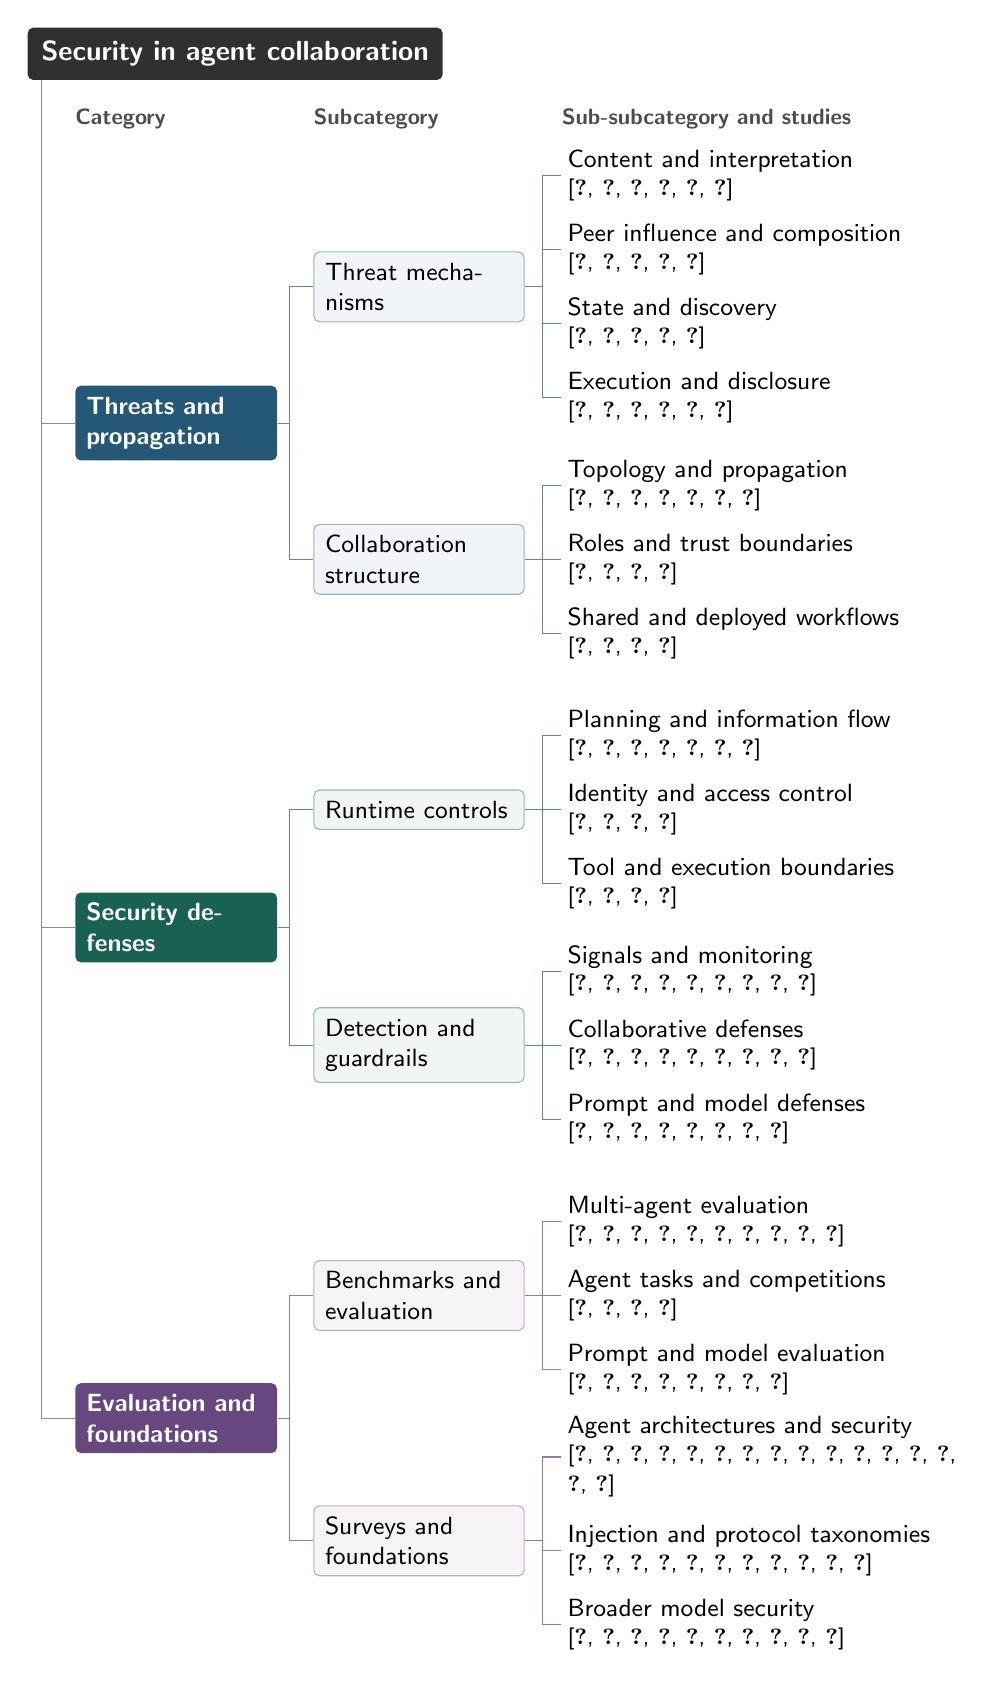
\begin{tikzpicture}[x=.01\linewidth,y=1cm,
  root/.style={anchor=west,rounded corners=2pt,fill=black!81,text=white,inner sep=5pt,font=\sffamily\bfseries},
  cat/.style={anchor=west,align=left,text width=.188\linewidth,inner sep=4pt,rounded corners=2pt,font=\sffamily\small\bfseries},
  sub/.style={anchor=west,align=left,text width=.197\linewidth,inner sep=4pt,rounded corners=2pt,font=\sffamily\small},
  leaf/.style={anchor=west,align=left,text width=.423\linewidth,inner sep=2pt,font=\sffamily\small},
  level/.style={anchor=west,font=\sffamily\footnotesize\bfseries,text=black!70,inner sep=0pt}]
\node[root] (root) at (0,1.42) {Security in agent collaboration};
\node[level] at (5,.59) {Category};
\node[level] at (30,.59) {Subcategory};
\node[level] at (56,.59) {Sub-subcategory and studies};
\definecolor{tier0}{HTML}{245876}
\definecolor{tier1}{HTML}{196253}
\definecolor{tier2}{HTML}{674780}
\coordinate (origin) at (1.5,.98);
\node[leaf] (leaf0) at (56,-0.130) {Content and interpretation\\[-1pt]{\footnotesize\cite{Gu2024AgentSAAO,Sehwag2026ASPISAAH,Yeo2025MultimodalPIBL,Pasquini2024NeuralELAL,greshake2023indirect,Wen2025RLIAU}}};
\node[leaf] (leaf1) at (56,-1.070) {Peer influence and composition\\[-1pt]{\footnotesize\cite{shahroz2025siege,Yan2025AttackTMAQ,arif2026conjunctive,lee2024promptinfection,he2025aitm}}};
\node[leaf] (leaf2) at (56,-2.010) {State and discovery\\[-1pt]{\footnotesize\cite{Chen2024AgentPoisonRLBS,Patlan2025CrossUserPUAK,Sunil2026MemoryPABF,Yu2026MisleadingTPO,Shi2025PromptIAR}}};
\node[leaf] (leaf3) at (56,-2.950) {Execution and disclosure\\[-1pt]{\footnotesize\cite{Pedro2023FromPIBE,Wang2025IPLAX,triedman2025mas,naik2026omnileak,Nagaraja2026WhenPCBF,Kao2026YouTMAZ}}};
\node[sub,fill=tier0!6,draw=tier0!45] (sub0) at (30,-1.540) {Threat mechanisms};
\coordinate (spine0) at (54,-1.540);
\node[leaf] (leaf4) at (56,-4.060) {Topology and propagation\\[-1pt]{\footnotesize\cite{hagag2026architecture,Hu2026AttackingADAX,Le2026CrosslayerCOAI,Malla2026FromMTI,Xie2026FromSTBA,Zhu2025MASTERMSR,Yu2025NetSafeETBB}}};
\node[leaf] (leaf5) at (56,-5.000) {Roles and trust boundaries\\[-1pt]{\footnotesize\cite{Paul2026BeyondSIE,peigne2025securitytax,Liu2026TheCPT,Mitra2026WhereREC}}};
\node[leaf] (leaf6) at (56,-5.940) {Shared and deployed workflows\\[-1pt]{\footnotesize\cite{Mitra2026AgenticCyOpsSMAH,Jamshidi2026SecurityEOAG,Wang2025ShadowsITAL,Nakamura2025TerrariumRTAR}}};
\node[sub,fill=tier0!6,draw=tier0!45] (sub1) at (30,-5.000) {Collaboration\\structure};
\coordinate (spine1) at (54,-5.000);
\node[cat,fill=tier0,text=white] (cat0) at (5,-3.270) {Threats and\\propagation};
\coordinate (split0) at (27.5,-3.270);
\node[leaf] (leaf7) at (56,-7.240) {Planning and information flow\\[-1pt]{\footnotesize\cite{Mao2025AgentSafeSLY,jha2025controlvalve,debenedetti2025camel,li2025drift,an2025ipiguard,wu2024ifc,Hu2026TwinACI}}};
\node[leaf] (leaf8) at (56,-8.180) {Identity and access control\\[-1pt]{\footnotesize\cite{Tallam2026AuthorizationPIBH,Zou2025BlockA2ATSAC,Narajala2025SecuringGMAU,Ji2026TamingVPAP}}};
\node[leaf] (leaf9) at (56,-9.120) {Tool and execution boundaries\\[-1pt]{\footnotesize\cite{Taheri2020MitigationARBP,Engelmann2022RV4JaCaRBL,Rashidi2026TheBOBQ,Li2026UniversalDFL}}};
\node[sub,fill=tier1!6,draw=tier1!45] (sub2) at (30,-8.180) {Runtime controls};
\coordinate (spine2) at (54,-8.180);
\node[leaf] (leaf10) at (56,-10.230) {Signals and monitoring\\[-1pt]{\footnotesize\cite{Malik2026ADLK,Cai2026CrossLayerSFBK,Alamsabi2026EmbeddingBasedDOX,Li2026MESAPVAS,Hashmi2026PromptIDBR,Shi2026SAIGuardCSN,Gosmar2025SentinelAFAJ,Xu2026WhenAGQ,Xie2025WhosTMAI}}};
\node[leaf] (leaf11) at (56,-11.170) {Collaborative defenses\\[-1pt]{\footnotesize\cite{Hossain2025AMLV,Miao2025BlindGuardSLAV,Luo2026DefendingLMV,Wang2025GSafeguardATAW,Kachuee2026MASGuardUGW,Wang2025MASShieldADAF,Zhang2026OpenEvoShieldDNZ,Gosmar2025PromptIDY,Yan2026PropGuardSLAE}}};
\node[leaf] (leaf12) at (56,-12.110) {Prompt and model defenses\\[-1pt]{\footnotesize\cite{Shaheer2025BeyondTBAW,Chen2024DefenseAPBG,Li2024InjecGuardBABC,Piet2023JatmoPIAS,li2025piguard,Gosmar2026PromptIMAA,Ramakrishnan2025SecuringAAAA,chen2025struq}}};
\node[sub,fill=tier1!6,draw=tier1!45] (sub3) at (30,-11.170) {Detection and guardrails};
\coordinate (spine3) at (54,-11.170);
\node[cat,fill=tier1,text=white] (cat1) at (5,-9.675) {Security defenses};
\coordinate (split1) at (27.5,-9.675);
\node[leaf] (leaf13) at (56,-13.410) {Multi-agent evaluation\\[-1pt]{\footnotesize\cite{An2026ACIArenaTUH,Ogunjinmi2026AgenticARN,Carolina2025EvaluatingMDAX,MateoTorrejon2026GAMMAFACAG,Liu2026MADBenchBTU,Hagag2026ORBITAFAD,Zhang2024PsySafeACAN,kavathekar2025tamas,Sharma2025TowardsUQBD,Wang2026TrinityGuardAUF}}};
\node[leaf] (leaf14) at (56,-14.350) {Agent tasks and competitions\\[-1pt]{\footnotesize\cite{zhang2025asb,Dziemian2026HowVAAN,zhan2024injecagent,Zou2025SecurityCIAD}}};
\node[leaf] (leaf15) at (56,-15.290) {Prompt and model evaluation\\[-1pt]{\footnotesize\cite{Yi2023BenchmarkingADAR,Wan2024CYBERSECEVAL3ABJ,liu2024formalizing,Li2024GenTelSafeAUAU,Liu2026LongPIBenchALAV,aal2025PromptIABT,Benjamin2024SystematicallyAPBK,Toyer2023TensorTIAM}}};
\node[sub,fill=tier2!6,draw=tier2!45] (sub4) at (30,-14.350) {Benchmarks and\\evaluation};
\coordinate (spine4) at (54,-14.350);
\node[leaf] (leaf16) at (56,-16.400) {Agent architectures and security\\[-1pt]{\footnotesize\cite{Shahriar2025ASOE,Yu2025ASOL,Siu2026AgentSNZ,Xiang2026ArchitectingSAAP,Zhu2026BlockchainETAT,Luo2025LargeLMBI,Hossain2026OnUIS,Witt2025OpenCIBE,Rafe2026OrchestrationAVK,Xu2026SecurityAAJ,Wang2025SecurityOIBN,Owoputi2022SecurityOMD,Yang2026SoKWSJ,RahulDevT2026TowardSAG,Ling2026TowardSLG,Li2026TowardsSABM}}};
\node[leaf] (leaf17) at (56,-17.590) {Injection and protocol taxonomies\\[-1pt]{\footnotesize\cite{Cao2026ASSM,Yadav2025AdversialPIBA,Song2025BeyondTPAE,Mao2025FromLTAY,Ferrag2025FromPIB,McHugh2025PromptI2F,Prabhakarn2026PromptIAAZ,Geng2025PromptIABB,Mourad2026SecuringTPAQ,Rababah2024SoKPHBH,Wang2026TheLOT}}};
\node[leaf] (leaf18) at (56,-18.530) {Broader model security\\[-1pt]{\footnotesize\cite{Xu2025ASOAT,Chowdhury2024BreakingDTBQ,Liu2024ExploringVABS,Ferrag2024GenerativeAIBM,Peng2024JailbreakingAMAY,S2025ModernDLAC,Cui2024RecentAIBO,Peng2024SecuringLLBR,Das2024SecurityAPBP,Li2025SecurityCFBN}}};
\node[sub,fill=tier2!6,draw=tier2!45] (sub5) at (30,-17.465) {Surveys and\\foundations};
\coordinate (spine5) at (54,-17.465);
\node[cat,fill=tier2,text=white] (cat2) at (5,-15.907) {Evaluation and foundations};
\coordinate (split2) at (27.5,-15.907);
\draw[tier0!72] (spine0) |- (leaf0.west);
\draw[tier0!72] (spine0) |- (leaf1.west);
\draw[tier0!72] (spine0) |- (leaf2.west);
\draw[tier0!72] (spine0) |- (leaf3.west);
\draw[tier0!72] (sub0.east)--(spine0);
\draw[tier0!72] (split0) |- (sub0.west);
\draw[tier0!72] (spine1) |- (leaf4.west);
\draw[tier0!72] (spine1) |- (leaf5.west);
\draw[tier0!72] (spine1) |- (leaf6.west);
\draw[tier0!72] (sub1.east)--(spine1);
\draw[tier0!72] (split0) |- (sub1.west);
\draw[tier0!72] (cat0.east)--(split0);
\draw[black!45] (origin) |- (cat0.west);
\draw[tier1!72] (spine2) |- (leaf7.west);
\draw[tier1!72] (spine2) |- (leaf8.west);
\draw[tier1!72] (spine2) |- (leaf9.west);
\draw[tier1!72] (sub2.east)--(spine2);
\draw[tier1!72] (split1) |- (sub2.west);
\draw[tier1!72] (spine3) |- (leaf10.west);
\draw[tier1!72] (spine3) |- (leaf11.west);
\draw[tier1!72] (spine3) |- (leaf12.west);
\draw[tier1!72] (sub3.east)--(spine3);
\draw[tier1!72] (split1) |- (sub3.west);
\draw[tier1!72] (cat1.east)--(split1);
\draw[black!45] (origin) |- (cat1.west);
\draw[tier2!72] (spine4) |- (leaf13.west);
\draw[tier2!72] (spine4) |- (leaf14.west);
\draw[tier2!72] (spine4) |- (leaf15.west);
\draw[tier2!72] (sub4.east)--(spine4);
\draw[tier2!72] (split2) |- (sub4.west);
\draw[tier2!72] (spine5) |- (leaf16.west);
\draw[tier2!72] (spine5) |- (leaf17.west);
\draw[tier2!72] (spine5) |- (leaf18.west);
\draw[tier2!72] (sub5.east)--(spine5);
\draw[tier2!72] (split2) |- (sub5.west);
\draw[tier2!72] (cat2.east)--(split2);
\draw[black!45] (origin) |- (cat2.west);
\draw[black!45] (origin |- root.south) -- (origin);
\end{tikzpicture}
\caption{Taxonomy of 137 studies by primary research focus. Each path connects a category to a subcategory and then to a cited sub-subcategory.}\label{fig:inert-corpus-tree}
\end{figure}
\clearpage
\ifdefined\INERTmanuscript\else
\bibliographystyle{plainnat}
\bibliography{injection_channel_taxonomy}
\fi
\ifdefined\INERTmanuscript\else\expandafter\enddocument\fi
.
\ifdefined\INERTmanuscript\else
\documentclass[11pt]{article}
\usepackage[margin=23mm]{geometry}
\usepackage[numbers,sort&compress]{natbib}
\usepackage{longtable,graphicx,tikz,booktabs,xurl}
\usepackage[colorlinks=true,citecolor=teal,urlcolor=teal,linkcolor=teal]{hyperref}
\setlength{\parindent}{0pt}\setlength{\parskip}{5pt}
\begin{document}
\fi
\section{A Taxonomy of Injection Channels in Agent Collaboration}\label{sec:taxonomy}

A reader agent may be authorized to summarize a document, a coordinator to assign work, and a publisher to release a report. The document can legitimately influence the report's contents. It becomes a security concern if text derived from that document can also determine who receives the report or whether it is released. The distinction turns on the authority of the receiving decision. Even a correctly authenticated summary can carry information whose original author had no authority over that decision~\citep{greshake2023indirect,triedman2025mas,debenedetti2025camel}.

\subsection{Unit of analysis and classification rule}

We define an \emph{injection channel} as a path by which externally influenced content reaches a component that can interpret it as an instruction or use it to make a protected decision. For each observed handoff we record the \emph{source} that supplied the content, the \emph{carrier} that conveyed it, the \emph{consumer} that interpreted it, and the \emph{decision} that the workflow authorizes that consumer to make. We also record the attacker's assumed access, how long the content remains available, and what the execution trace actually establishes. An origin such as a compromised worker describes who can act. An outcome such as disclosure describes what happened. Either can occur across several channels.

Table~\ref{tab:channels-inert} classifies each handoff by the interface through which the receiving component obtains the content. A run can cross several interfaces. For example, a document read from an issue tracker, summarized by a worker, and retained for a later session crosses the external-content, peer-message, and shared-state channels in sequence. If the summary is later read to choose a recipient, that last use is a protected decision. Counting each handoff retains both the original source and the later point at which the application grants the value authority. This decomposition complements existing taxonomies of entry points and multi-agent attack paths~\citep{Mitra2026WhereREC,Yang2026SoKWSJ,Paul2026BeyondSIE}.


\begin{longtable}{@{}p{.16\linewidth}@{\hspace{.02\linewidth}}p{.25\linewidth}@{\hspace{.02\linewidth}}p{.27\linewidth}@{\hspace{.02\linewidth}}p{.25\linewidth}@{}}
\caption{Injection channels classified by receiving interface. The final column gives an example of a policy obligation a developer can express and check.}\label{tab:channels-inert}\\
\hline\textbf{Channel} & \textbf{Source and carrier} & \textbf{Consumer and decision} & \textbf{Example obligation}\\\hline\endfirsthead
\hline\textbf{Channel} & \textbf{Source and carrier} & \textbf{Consumer and decision} & \textbf{Example obligation}\\\hline\endhead
User request & A caller supplies a task, clarification, or conversational reply. & An intake agent interprets the request and chooses its scope. & Bind each request to its principal, task, and permitted operations.\\[3pt]
External content & An external author supplies a document, issue, email, or image that an agent retrieves. & A reader extracts facts that may later influence other agents. & Retrieved content may populate report text. Release approval requires an independent authorized source.\\[3pt]
Tool response & A service returns data or diagnostic text from a permitted tool call. & A worker interprets the result, or a coordinator uses reported status to select a next step. & Bind the response to its invocation. Validate control-relevant status separately from free text.\\[3pt]
Peer message & A worker, reviewer, or intermediary supplies a message, summary, or proposed value. & A peer incorporates the value into its reasoning or output. & Check sender, role, request, and permitted dependencies of the receiving field.\\[3pt]
Coordination signal & An agent reports completion, failure, a review verdict, or a delegation request. & An orchestrator chooses a transition, successor, retry, or release. & Accept only authorized transitions for the current workflow state and request.\\[3pt]
Shared state & A prior task, peer, or external writer contributes a memory, blackboard item, or knowledge-base record. & A later retrieval introduces the value into a new decision context. & Scope reads by principal and task, and retain the provenance of retrieved values.\\[3pt]
Discovery metadata & A provider publishes an agent description, skill declaration, or tool record. & A planner or registry resolves a name, selects a provider, or grants a capability. & Bind the approved identity and metadata version to the invocation.\\\hline
\end{longtable}

\subsection{Propagation, authority, and observable effects}

A peer message and a coordination signal can share the same transport. The distinction is the recipient's use of the field. A worker's narrative about a failed read is a peer message. A failure status that the controller accepts as authority to change the next step is a coordination signal. Likewise, an email returned by a tool has an external author and a tool-response envelope. Recording both avoids attributing the authority of the tool service to the author of the email. Registration-time influence occurs earlier still, when the planner first learns what a participant claims it can do~\citep{Yu2026MisleadingTPO}.

Three properties cut across the channels. First, influence can survive a transformation. A summary can preserve a request's meaning after its wording changes, and independently innocuous fragments can acquire a different meaning when agents combine them~\citep{lee2024promptinfection,arif2026conjunctive}. Second, the influence can outlive the interaction. Work on poisoned retrieval and cross-user context motivates recording which task wrote a value and which task subsequently read it~\citep{Chen2024AgentPoisonRLBS,Patlan2025CrossUserPUAK}. Third, authority can change along the path. A read-only worker can influence a peer with publishing privileges. The roles, topology, and memory visible to each agent therefore matter even when the agents use the same underlying model~\citep{hagag2026architecture,naik2026omnileak}.

For each boundary we distinguish \emph{exposure}, when a consumer receives the value, \emph{proposal}, when a component requests an action, \emph{acceptance}, when a controller authorizes it, and \emph{effect}, when there is evidence of a disclosure or state change. A denied proposal and a successful disclosure warrant different verdicts. A record that an executor accepted a request establishes acceptance. Establishing delivery to an external recipient may also require a service receipt or observable state change. A malicious participant that directly misuses an allowed tool is an important comparison case: attribution to injection requires evidence of an influencing input~\citep{kavathekar2025tamas}.

\subsection{Evidence from the studies}

Table~\ref{tab:channel-evidence} decomposes the studies that anchor the channel definitions. Its last column gives our interpretation of the evidence for a workflow designer. Benchmarks supply defined scenarios, architecture studies vary system choices, and defense papers identify potential enforcement points. These forms of evidence support different conclusions. In particular, a defense evaluated on tool-response injection does not by itself establish protection against a compromised participant or a value retrieved by another user.

\begin{longtable}{@{}p{.19\linewidth}@{\hspace{.02\linewidth}}p{.22\linewidth}@{\hspace{.02\linewidth}}p{.24\linewidth}@{\hspace{.02\linewidth}}p{.28\linewidth}@{}}
\caption{Study-level evidence. The study design appears beneath each citation. Carrier, receiving decision, and implication are coded separately.}\label{tab:channel-evidence}\\
\hline\textbf{Study} & \textbf{Source and carrier} & \textbf{Consumer or decision} & \textbf{Implication for testing}\\\hline\endfirsthead
\hline\textbf{Study} & \textbf{Source and carrier} & \textbf{Consumer or decision} & \textbf{Implication for testing}\\\hline\endhead
Indirect injection~\citep{greshake2023indirect}\par{\footnotesize\itshape Application case studies} & External author, retrieved content & Application reads data for a legitimate task & The document author and the caller can have different authority.\\[3pt]
InjecAgent~\citep{zhan2024injecagent}\par{\footnotesize\itshape Tool-use benchmark} & Tool service, returned content & Agent considers a subsequent tool action & A permitted read can expose an agent to unauthorized instructions.\\[3pt]
Email-agent detection~\citep{Hashmi2026PromptIDBR}\par{\footnotesize\itshape Email-agent detection study} & Email author, message content & Email agent processes a sequence of events & The email is an entry point; later decisions determine the effect.\\[3pt]
Prompt Infection~\citep{lee2024promptinfection}\par{\footnotesize\itshape Propagation experiments} & Peer, generated message & Other agents consume and reproduce instructions & Record each receiving agent, including peers that only relay content.\\[3pt]
Agent-in-the-Middle~\citep{he2025aitm}\par{\footnotesize\itshape Communication threat model} & Intermediary, inter-agent message & Recipient reads a modified message & Message integrity and sender authorization require separate checks.\\[3pt]
Conjunctive prompts~\citep{arif2026conjunctive}\par{\footnotesize\itshape Composition experiments} & Multiple inputs, routed segments & A downstream component combines context & A component-level verdict can miss a property of the combined input.\\[3pt]
Control-flow hijacking~\citep{triedman2025mas}\par{\footnotesize\itshape Orchestration experiments} & External content, reported status & Orchestrator selects a privileged next step & Record the transition and its authorizing evidence.\\[3pt]
ControlValve~\citep{jha2025controlvalve}\par{\footnotesize\itshape Control-flow defense} & Coordinator, invocation request & Controller checks graph and contextual rules & An allowed edge and an allowed invocation context are distinct obligations.\\[3pt]
Registration-time injection~\citep{Yu2026MisleadingTPO}\par{\footnotesize\itshape Planner-registration study} & Provider, worker description & Central planner chooses a worker & Provider-supplied claims can influence delegation before task execution.\\[3pt]
Tool squatting~\citep{Narajala2025SecuringGMAU}\par{\footnotesize\itshape Registry-based defense} & Provider, tool registration & Registry or planner resolves tool identity & Test identity resolution separately from authorization of arguments.\\[3pt]
AgentPoison~\citep{Chen2024AgentPoisonRLBS}\par{\footnotesize\itshape Retrieval-poisoning study} & External writer, persistent memory & Retriever brings a stored record into context & Record write provenance as well as the later retrieval.\\[3pt]
Cross-user poisoning~\citep{Patlan2025CrossUserPUAK}\par{\footnotesize\itshape Cross-user threat model} & Different principal, shared history & Shared agent acts in another task context & The identity of the current user is part of the authorization decision.\\[3pt]
Terrarium~\citep{Nakamura2025TerrariumRTAR}\par{\footnotesize\itshape Blackboard research framework} & Participants, shared blackboard & Agents read and contribute shared state & A shared-store model makes reads and writes explicit.\\[3pt]
OMNI-LEAK~\citep{naik2026omnileak}\par{\footnotesize\itshape Confidentiality study} & Multiple agents, cross-role data & Sensitive data reaches an external communication capability & Audit the destination and the provenance of released data.\\[3pt]
Architecture Matters~\citep{hagag2026architecture}\par{\footnotesize\itshape Architecture comparison} & Role, topology, memory visibility & Architecture changes opportunities for exposure and action & Compare stage-specific outcomes across architectures.\\[3pt]
TAMAS~\citep{kavathekar2025tamas}\par{\footnotesize\itshape Multi-agent benchmark} & External input or compromised participant & Agents interact across benchmark configurations & Stratify by attacker placement and retain benign utility.\\[3pt]
ACIArena~\citep{An2026ACIArenaTUH}\par{\footnotesize\itshape Cascading-injection benchmark} & External inputs, agent profiles, peer messages & Benchmark tracks instruction hijacking, task disruption, and disclosure & Its 1,356 cases across six implementations separate the entry surface from the attack objective.\\[3pt]
Judgment boundary~\citep{Mitra2026WhereREC}\par{\footnotesize\itshape Layered policy evaluation} & Multiple entry points, policy-relevant inputs & Layered checks and judgments mediate decisions & Identify which verdicts follow from explicit rules and which require interpretation.\\[3pt]
CaMeL~\citep{debenedetti2025camel}\par{\footnotesize\itshape Information-flow defense} & Untrusted data, tool arguments & Program interpreter checks authorized flows & A fixed plan still needs a policy for values reaching tool calls.\\[3pt]
DRIFT~\citep{li2025drift}\par{\footnotesize\itshape Runtime defense} & Tool interactions, memory stream & Validator and isolator mediate evolving context & A change in permissions and a persistent record require different checks.\\[3pt]
Robotic systems~\citep{Nagaraja2026WhenPCBF}\par{\footnotesize\itshape Robotic task evaluation} & Agent inputs, multi-agent decisions & Robotic task execution can exhibit unintended behavior & Define the effect in the application's observable state.\\[3pt]
\hline\end{longtable}

\subsection{From channel categories to model-based test obligations}

For each modeled channel, a developer can identify a permitted use, a protected decision, and an observable event that distinguishes them. In the report workflow, a positive test checks that document-derived text may enter the summary. A companion test checks whether a value with that same provenance can become release approval. A third checks whether the authorized reviewer can still approve the current report. The three observations distinguish successful task execution, enforcement of the source restriction, and an overly restrictive policy that suppresses useful work.

The structural obligations concern the identity of the sender, the current request, the selected transition, and the tool bound to the invocation. Information-flow obligations concern the dependencies of the accepted value. A permitted author can still submit a value derived from a disallowed source. Conversely, an agent can submit a well-typed but factually wrong summary within its authority. INERT checks the modeled permissions and dependencies; factual correctness requires an appropriate content oracle. Coverage is relative to the declared model, and an observed run supplies evidence only about the events visible to its oracle. This interpretation connects scenario-based evaluation and structural workflow coverage to the generation criteria in the test-generation section~\citep{debenedetti2024agentdojo,kahani2026structural}.


Table~\ref{tab:channel-oracles} gives paired observations for the seven interfaces. The examples specify what an evaluator would need to observe. They are proposed test obligations derived from the taxonomy.

\begin{longtable}{@{}p{.16\linewidth}@{\hspace{.02\linewidth}}p{.25\linewidth}@{\hspace{.02\linewidth}}p{.25\linewidth}@{\hspace{.02\linewidth}}p{.27\linewidth}@{}}
\caption{Channel-specific evidence for authority, benign utility, and policy violations. Each row describes one possible policy and its oracle.}\label{tab:channel-oracles}\\
\toprule\textbf{Interface} & \textbf{Binding to record} & \textbf{Benign witness} & \textbf{Violation witness}\\\midrule\endfirsthead
\toprule\textbf{Interface} & \textbf{Binding to record} & \textbf{Benign witness} & \textbf{Violation witness}\\\midrule\endhead
User request & Caller identity, task owner, active request. & A caller revises a task that they own. & A revision is committed to another principal's task without delegated authority.\\[4pt]
External content & Document identity, derived fields, release policy. & The report includes facts from the retrieved document. & Release approval is accepted from a value derived solely from document text.\\[4pt]
Tool response & Call identifier, expected responder, status field. & A result updates the field requested by the pending call. & A result for an earlier call is accepted as the current call's completion.\\[4pt]
Peer message & Authorized author, destination field, request version. & The assigned reviewer supplies a verdict for the current revision. & A different peer or a stale review fills the protected verdict field.\\[4pt]
Coordination signal & Current workflow state, transition, role required to authorize it. & A valid review advances the current report to release. & A release transition occurs without an accepted review for that report.\\[4pt]
Shared state & Record writer, owner, visibility, task of subsequent read. & A worker retrieves its own task's permitted notes. & A private record from another task appears in the worker's delivered context.\\[4pt]
Discovery metadata & Approved provider identity, descriptor version, resolved executable. & The dispatcher invokes the provider and version approved for the task. & The dispatcher binds the invocation to a provider outside the approved set.\\[4pt]
\bottomrule\end{longtable}

\subsection{Research branches represented in the corpus}

Figure~\ref{fig:inert-corpus-tree} classifies the indexed literature by primary research focus. For example, a study of how one agent's message influences another follows the path from threats and propagation to threat mechanisms and then to peer influence and composition. Each study appears at one leaf.

\begin{figure}[p]
\centering
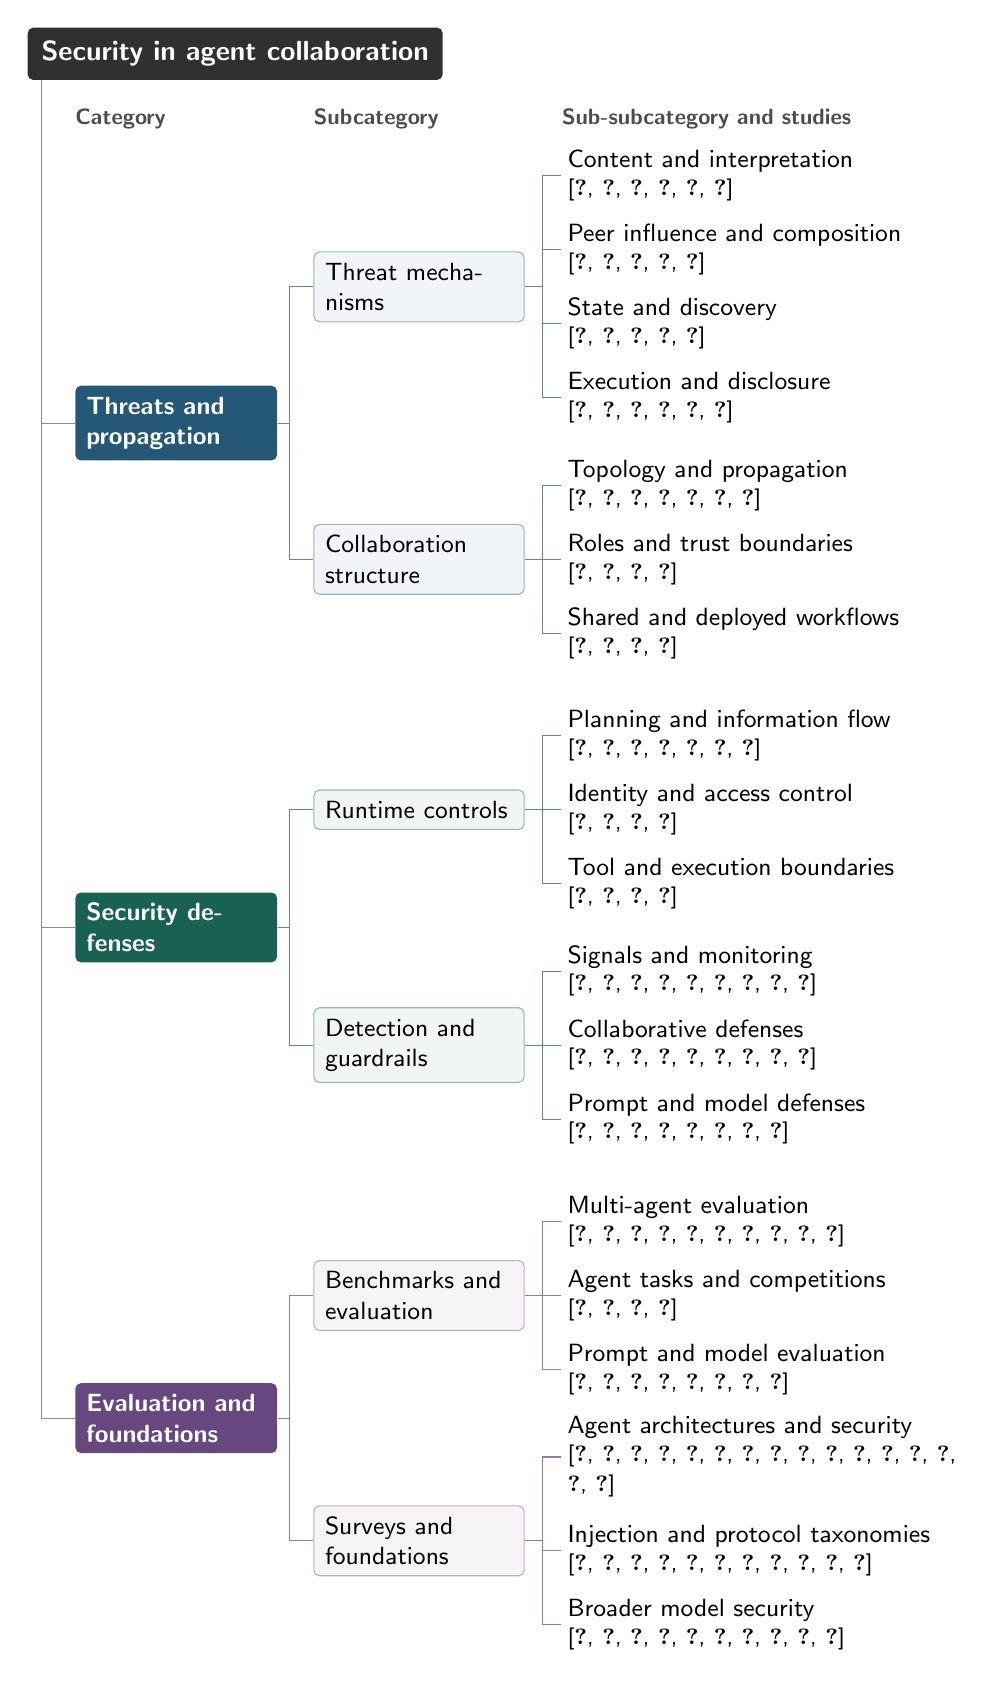
\begin{tikzpicture}[x=.01\linewidth,y=1cm,
  root/.style={anchor=west,rounded corners=2pt,fill=black!81,text=white,inner sep=5pt,font=\sffamily\bfseries},
  cat/.style={anchor=west,align=left,text width=.188\linewidth,inner sep=4pt,rounded corners=2pt,font=\sffamily\small\bfseries},
  sub/.style={anchor=west,align=left,text width=.197\linewidth,inner sep=4pt,rounded corners=2pt,font=\sffamily\small},
  leaf/.style={anchor=west,align=left,text width=.423\linewidth,inner sep=2pt,font=\sffamily\small},
  level/.style={anchor=west,font=\sffamily\footnotesize\bfseries,text=black!70,inner sep=0pt}]
\node[root] (root) at (0,1.42) {Security in agent collaboration};
\node[level] at (5,.59) {Category};
\node[level] at (30,.59) {Subcategory};
\node[level] at (56,.59) {Sub-subcategory and studies};
\definecolor{tier0}{HTML}{245876}
\definecolor{tier1}{HTML}{196253}
\definecolor{tier2}{HTML}{674780}
\coordinate (origin) at (1.5,.98);
\node[leaf] (leaf0) at (56,-0.130) {Content and interpretation\\[-1pt]{\footnotesize\cite{Gu2024AgentSAAO,Sehwag2026ASPISAAH,Yeo2025MultimodalPIBL,Pasquini2024NeuralELAL,greshake2023indirect,Wen2025RLIAU}}};
\node[leaf] (leaf1) at (56,-1.070) {Peer influence and composition\\[-1pt]{\footnotesize\cite{shahroz2025siege,Yan2025AttackTMAQ,arif2026conjunctive,lee2024promptinfection,he2025aitm}}};
\node[leaf] (leaf2) at (56,-2.010) {State and discovery\\[-1pt]{\footnotesize\cite{Chen2024AgentPoisonRLBS,Patlan2025CrossUserPUAK,Sunil2026MemoryPABF,Yu2026MisleadingTPO,Shi2025PromptIAR}}};
\node[leaf] (leaf3) at (56,-2.950) {Execution and disclosure\\[-1pt]{\footnotesize\cite{Pedro2023FromPIBE,Wang2025IPLAX,triedman2025mas,naik2026omnileak,Nagaraja2026WhenPCBF,Kao2026YouTMAZ}}};
\node[sub,fill=tier0!6,draw=tier0!45] (sub0) at (30,-1.540) {Threat mechanisms};
\coordinate (spine0) at (54,-1.540);
\node[leaf] (leaf4) at (56,-4.060) {Topology and propagation\\[-1pt]{\footnotesize\cite{hagag2026architecture,Hu2026AttackingADAX,Le2026CrosslayerCOAI,Malla2026FromMTI,Xie2026FromSTBA,Zhu2025MASTERMSR,Yu2025NetSafeETBB}}};
\node[leaf] (leaf5) at (56,-5.000) {Roles and trust boundaries\\[-1pt]{\footnotesize\cite{Paul2026BeyondSIE,peigne2025securitytax,Liu2026TheCPT,Mitra2026WhereREC}}};
\node[leaf] (leaf6) at (56,-5.940) {Shared and deployed workflows\\[-1pt]{\footnotesize\cite{Mitra2026AgenticCyOpsSMAH,Jamshidi2026SecurityEOAG,Wang2025ShadowsITAL,Nakamura2025TerrariumRTAR}}};
\node[sub,fill=tier0!6,draw=tier0!45] (sub1) at (30,-5.000) {Collaboration\\structure};
\coordinate (spine1) at (54,-5.000);
\node[cat,fill=tier0,text=white] (cat0) at (5,-3.270) {Threats and\\propagation};
\coordinate (split0) at (27.5,-3.270);
\node[leaf] (leaf7) at (56,-7.240) {Planning and information flow\\[-1pt]{\footnotesize\cite{Mao2025AgentSafeSLY,jha2025controlvalve,debenedetti2025camel,li2025drift,an2025ipiguard,wu2024ifc,Hu2026TwinACI}}};
\node[leaf] (leaf8) at (56,-8.180) {Identity and access control\\[-1pt]{\footnotesize\cite{Tallam2026AuthorizationPIBH,Zou2025BlockA2ATSAC,Narajala2025SecuringGMAU,Ji2026TamingVPAP}}};
\node[leaf] (leaf9) at (56,-9.120) {Tool and execution boundaries\\[-1pt]{\footnotesize\cite{Taheri2020MitigationARBP,Engelmann2022RV4JaCaRBL,Rashidi2026TheBOBQ,Li2026UniversalDFL}}};
\node[sub,fill=tier1!6,draw=tier1!45] (sub2) at (30,-8.180) {Runtime controls};
\coordinate (spine2) at (54,-8.180);
\node[leaf] (leaf10) at (56,-10.230) {Signals and monitoring\\[-1pt]{\footnotesize\cite{Malik2026ADLK,Cai2026CrossLayerSFBK,Alamsabi2026EmbeddingBasedDOX,Li2026MESAPVAS,Hashmi2026PromptIDBR,Shi2026SAIGuardCSN,Gosmar2025SentinelAFAJ,Xu2026WhenAGQ,Xie2025WhosTMAI}}};
\node[leaf] (leaf11) at (56,-11.170) {Collaborative defenses\\[-1pt]{\footnotesize\cite{Hossain2025AMLV,Miao2025BlindGuardSLAV,Luo2026DefendingLMV,Wang2025GSafeguardATAW,Kachuee2026MASGuardUGW,Wang2025MASShieldADAF,Zhang2026OpenEvoShieldDNZ,Gosmar2025PromptIDY,Yan2026PropGuardSLAE}}};
\node[leaf] (leaf12) at (56,-12.110) {Prompt and model defenses\\[-1pt]{\footnotesize\cite{Shaheer2025BeyondTBAW,Chen2024DefenseAPBG,Li2024InjecGuardBABC,Piet2023JatmoPIAS,li2025piguard,Gosmar2026PromptIMAA,Ramakrishnan2025SecuringAAAA,chen2025struq}}};
\node[sub,fill=tier1!6,draw=tier1!45] (sub3) at (30,-11.170) {Detection and guardrails};
\coordinate (spine3) at (54,-11.170);
\node[cat,fill=tier1,text=white] (cat1) at (5,-9.675) {Security defenses};
\coordinate (split1) at (27.5,-9.675);
\node[leaf] (leaf13) at (56,-13.410) {Multi-agent evaluation\\[-1pt]{\footnotesize\cite{An2026ACIArenaTUH,Ogunjinmi2026AgenticARN,Carolina2025EvaluatingMDAX,MateoTorrejon2026GAMMAFACAG,Liu2026MADBenchBTU,Hagag2026ORBITAFAD,Zhang2024PsySafeACAN,kavathekar2025tamas,Sharma2025TowardsUQBD,Wang2026TrinityGuardAUF}}};
\node[leaf] (leaf14) at (56,-14.350) {Agent tasks and competitions\\[-1pt]{\footnotesize\cite{zhang2025asb,Dziemian2026HowVAAN,zhan2024injecagent,Zou2025SecurityCIAD}}};
\node[leaf] (leaf15) at (56,-15.290) {Prompt and model evaluation\\[-1pt]{\footnotesize\cite{Yi2023BenchmarkingADAR,Wan2024CYBERSECEVAL3ABJ,liu2024formalizing,Li2024GenTelSafeAUAU,Liu2026LongPIBenchALAV,aal2025PromptIABT,Benjamin2024SystematicallyAPBK,Toyer2023TensorTIAM}}};
\node[sub,fill=tier2!6,draw=tier2!45] (sub4) at (30,-14.350) {Benchmarks and\\evaluation};
\coordinate (spine4) at (54,-14.350);
\node[leaf] (leaf16) at (56,-16.400) {Agent architectures and security\\[-1pt]{\footnotesize\cite{Shahriar2025ASOE,Yu2025ASOL,Siu2026AgentSNZ,Xiang2026ArchitectingSAAP,Zhu2026BlockchainETAT,Luo2025LargeLMBI,Hossain2026OnUIS,Witt2025OpenCIBE,Rafe2026OrchestrationAVK,Xu2026SecurityAAJ,Wang2025SecurityOIBN,Owoputi2022SecurityOMD,Yang2026SoKWSJ,RahulDevT2026TowardSAG,Ling2026TowardSLG,Li2026TowardsSABM}}};
\node[leaf] (leaf17) at (56,-17.590) {Injection and protocol taxonomies\\[-1pt]{\footnotesize\cite{Cao2026ASSM,Yadav2025AdversialPIBA,Song2025BeyondTPAE,Mao2025FromLTAY,Ferrag2025FromPIB,McHugh2025PromptI2F,Prabhakarn2026PromptIAAZ,Geng2025PromptIABB,Mourad2026SecuringTPAQ,Rababah2024SoKPHBH,Wang2026TheLOT}}};
\node[leaf] (leaf18) at (56,-18.530) {Broader model security\\[-1pt]{\footnotesize\cite{Xu2025ASOAT,Chowdhury2024BreakingDTBQ,Liu2024ExploringVABS,Ferrag2024GenerativeAIBM,Peng2024JailbreakingAMAY,S2025ModernDLAC,Cui2024RecentAIBO,Peng2024SecuringLLBR,Das2024SecurityAPBP,Li2025SecurityCFBN}}};
\node[sub,fill=tier2!6,draw=tier2!45] (sub5) at (30,-17.465) {Surveys and\\foundations};
\coordinate (spine5) at (54,-17.465);
\node[cat,fill=tier2,text=white] (cat2) at (5,-15.907) {Evaluation and foundations};
\coordinate (split2) at (27.5,-15.907);
\draw[tier0!72] (spine0) |- (leaf0.west);
\draw[tier0!72] (spine0) |- (leaf1.west);
\draw[tier0!72] (spine0) |- (leaf2.west);
\draw[tier0!72] (spine0) |- (leaf3.west);
\draw[tier0!72] (sub0.east)--(spine0);
\draw[tier0!72] (split0) |- (sub0.west);
\draw[tier0!72] (spine1) |- (leaf4.west);
\draw[tier0!72] (spine1) |- (leaf5.west);
\draw[tier0!72] (spine1) |- (leaf6.west);
\draw[tier0!72] (sub1.east)--(spine1);
\draw[tier0!72] (split0) |- (sub1.west);
\draw[tier0!72] (cat0.east)--(split0);
\draw[black!45] (origin) |- (cat0.west);
\draw[tier1!72] (spine2) |- (leaf7.west);
\draw[tier1!72] (spine2) |- (leaf8.west);
\draw[tier1!72] (spine2) |- (leaf9.west);
\draw[tier1!72] (sub2.east)--(spine2);
\draw[tier1!72] (split1) |- (sub2.west);
\draw[tier1!72] (spine3) |- (leaf10.west);
\draw[tier1!72] (spine3) |- (leaf11.west);
\draw[tier1!72] (spine3) |- (leaf12.west);
\draw[tier1!72] (sub3.east)--(spine3);
\draw[tier1!72] (split1) |- (sub3.west);
\draw[tier1!72] (cat1.east)--(split1);
\draw[black!45] (origin) |- (cat1.west);
\draw[tier2!72] (spine4) |- (leaf13.west);
\draw[tier2!72] (spine4) |- (leaf14.west);
\draw[tier2!72] (spine4) |- (leaf15.west);
\draw[tier2!72] (sub4.east)--(spine4);
\draw[tier2!72] (split2) |- (sub4.west);
\draw[tier2!72] (spine5) |- (leaf16.west);
\draw[tier2!72] (spine5) |- (leaf17.west);
\draw[tier2!72] (spine5) |- (leaf18.west);
\draw[tier2!72] (sub5.east)--(spine5);
\draw[tier2!72] (split2) |- (sub5.west);
\draw[tier2!72] (cat2.east)--(split2);
\draw[black!45] (origin) |- (cat2.west);
\draw[black!45] (origin |- root.south) -- (origin);
\end{tikzpicture}
\caption{Taxonomy of 137 studies by primary research focus. Each path connects a category to a subcategory and then to a cited sub-subcategory.}\label{fig:inert-corpus-tree}
\end{figure}
\clearpage
\ifdefined\INERTmanuscript\else
\bibliographystyle{plainnat}
\bibliography{injection_channel_taxonomy}
\fi
\ifdefined\INERTmanuscript\else\expandafter\enddocument\fi
.
\ifdefined\INERTmanuscript\else
\documentclass[11pt]{article}
\usepackage[margin=23mm]{geometry}
\usepackage[numbers,sort&compress]{natbib}
\usepackage{longtable,graphicx,tikz,booktabs,xurl}
\usepackage[colorlinks=true,citecolor=teal,urlcolor=teal,linkcolor=teal]{hyperref}
\setlength{\parindent}{0pt}\setlength{\parskip}{5pt}
\begin{document}
\fi
\section{A Taxonomy of Injection Channels in Agent Collaboration}\label{sec:taxonomy}

A reader agent may be authorized to summarize a document, a coordinator to assign work, and a publisher to release a report. The document can legitimately influence the report's contents. It becomes a security concern if text derived from that document can also determine who receives the report or whether it is released. The distinction turns on the authority of the receiving decision. Even a correctly authenticated summary can carry information whose original author had no authority over that decision~\citep{greshake2023indirect,triedman2025mas,debenedetti2025camel}.

\subsection{Unit of analysis and classification rule}

We define an \emph{injection channel} as a path by which externally influenced content reaches a component that can interpret it as an instruction or use it to make a protected decision. For each observed handoff we record the \emph{source} that supplied the content, the \emph{carrier} that conveyed it, the \emph{consumer} that interpreted it, and the \emph{decision} that the workflow authorizes that consumer to make. We also record the attacker's assumed access, how long the content remains available, and what the execution trace actually establishes. An origin such as a compromised worker describes who can act. An outcome such as disclosure describes what happened. Either can occur across several channels.

Table~\ref{tab:channels-inert} classifies each handoff by the interface through which the receiving component obtains the content. A run can cross several interfaces. For example, a document read from an issue tracker, summarized by a worker, and retained for a later session crosses the external-content, peer-message, and shared-state channels in sequence. If the summary is later read to choose a recipient, that last use is a protected decision. Counting each handoff retains both the original source and the later point at which the application grants the value authority. This decomposition complements existing taxonomies of entry points and multi-agent attack paths~\citep{Mitra2026WhereREC,Yang2026SoKWSJ,Paul2026BeyondSIE}.


\begin{longtable}{@{}p{.16\linewidth}@{\hspace{.02\linewidth}}p{.25\linewidth}@{\hspace{.02\linewidth}}p{.27\linewidth}@{\hspace{.02\linewidth}}p{.25\linewidth}@{}}
\caption{Injection channels classified by receiving interface. The final column gives an example of a policy obligation a developer can express and check.}\label{tab:channels-inert}\\
\hline\textbf{Channel} & \textbf{Source and carrier} & \textbf{Consumer and decision} & \textbf{Example obligation}\\\hline\endfirsthead
\hline\textbf{Channel} & \textbf{Source and carrier} & \textbf{Consumer and decision} & \textbf{Example obligation}\\\hline\endhead
User request & A caller supplies a task, clarification, or conversational reply. & An intake agent interprets the request and chooses its scope. & Bind each request to its principal, task, and permitted operations.\\[3pt]
External content & An external author supplies a document, issue, email, or image that an agent retrieves. & A reader extracts facts that may later influence other agents. & Retrieved content may populate report text. Release approval requires an independent authorized source.\\[3pt]
Tool response & A service returns data or diagnostic text from a permitted tool call. & A worker interprets the result, or a coordinator uses reported status to select a next step. & Bind the response to its invocation. Validate control-relevant status separately from free text.\\[3pt]
Peer message & A worker, reviewer, or intermediary supplies a message, summary, or proposed value. & A peer incorporates the value into its reasoning or output. & Check sender, role, request, and permitted dependencies of the receiving field.\\[3pt]
Coordination signal & An agent reports completion, failure, a review verdict, or a delegation request. & An orchestrator chooses a transition, successor, retry, or release. & Accept only authorized transitions for the current workflow state and request.\\[3pt]
Shared state & A prior task, peer, or external writer contributes a memory, blackboard item, or knowledge-base record. & A later retrieval introduces the value into a new decision context. & Scope reads by principal and task, and retain the provenance of retrieved values.\\[3pt]
Discovery metadata & A provider publishes an agent description, skill declaration, or tool record. & A planner or registry resolves a name, selects a provider, or grants a capability. & Bind the approved identity and metadata version to the invocation.\\\hline
\end{longtable}

\subsection{Propagation, authority, and observable effects}

A peer message and a coordination signal can share the same transport. The distinction is the recipient's use of the field. A worker's narrative about a failed read is a peer message. A failure status that the controller accepts as authority to change the next step is a coordination signal. Likewise, an email returned by a tool has an external author and a tool-response envelope. Recording both avoids attributing the authority of the tool service to the author of the email. Registration-time influence occurs earlier still, when the planner first learns what a participant claims it can do~\citep{Yu2026MisleadingTPO}.

Three properties cut across the channels. First, influence can survive a transformation. A summary can preserve a request's meaning after its wording changes, and independently innocuous fragments can acquire a different meaning when agents combine them~\citep{lee2024promptinfection,arif2026conjunctive}. Second, the influence can outlive the interaction. Work on poisoned retrieval and cross-user context motivates recording which task wrote a value and which task subsequently read it~\citep{Chen2024AgentPoisonRLBS,Patlan2025CrossUserPUAK}. Third, authority can change along the path. A read-only worker can influence a peer with publishing privileges. The roles, topology, and memory visible to each agent therefore matter even when the agents use the same underlying model~\citep{hagag2026architecture,naik2026omnileak}.

For each boundary we distinguish \emph{exposure}, when a consumer receives the value, \emph{proposal}, when a component requests an action, \emph{acceptance}, when a controller authorizes it, and \emph{effect}, when there is evidence of a disclosure or state change. A denied proposal and a successful disclosure warrant different verdicts. A record that an executor accepted a request establishes acceptance. Establishing delivery to an external recipient may also require a service receipt or observable state change. A malicious participant that directly misuses an allowed tool is an important comparison case: attribution to injection requires evidence of an influencing input~\citep{kavathekar2025tamas}.

\subsection{Evidence from the studies}

Table~\ref{tab:channel-evidence} decomposes the studies that anchor the channel definitions. Its last column gives our interpretation of the evidence for a workflow designer. Benchmarks supply defined scenarios, architecture studies vary system choices, and defense papers identify potential enforcement points. These forms of evidence support different conclusions. In particular, a defense evaluated on tool-response injection does not by itself establish protection against a compromised participant or a value retrieved by another user.

\begin{longtable}{@{}p{.19\linewidth}@{\hspace{.02\linewidth}}p{.22\linewidth}@{\hspace{.02\linewidth}}p{.24\linewidth}@{\hspace{.02\linewidth}}p{.28\linewidth}@{}}
\caption{Study-level evidence. The study design appears beneath each citation. Carrier, receiving decision, and implication are coded separately.}\label{tab:channel-evidence}\\
\hline\textbf{Study} & \textbf{Source and carrier} & \textbf{Consumer or decision} & \textbf{Implication for testing}\\\hline\endfirsthead
\hline\textbf{Study} & \textbf{Source and carrier} & \textbf{Consumer or decision} & \textbf{Implication for testing}\\\hline\endhead
Indirect injection~\citep{greshake2023indirect}\par{\footnotesize\itshape Application case studies} & External author, retrieved content & Application reads data for a legitimate task & The document author and the caller can have different authority.\\[3pt]
InjecAgent~\citep{zhan2024injecagent}\par{\footnotesize\itshape Tool-use benchmark} & Tool service, returned content & Agent considers a subsequent tool action & A permitted read can expose an agent to unauthorized instructions.\\[3pt]
Email-agent detection~\citep{Hashmi2026PromptIDBR}\par{\footnotesize\itshape Email-agent detection study} & Email author, message content & Email agent processes a sequence of events & The email is an entry point; later decisions determine the effect.\\[3pt]
Prompt Infection~\citep{lee2024promptinfection}\par{\footnotesize\itshape Propagation experiments} & Peer, generated message & Other agents consume and reproduce instructions & Record each receiving agent, including peers that only relay content.\\[3pt]
Agent-in-the-Middle~\citep{he2025aitm}\par{\footnotesize\itshape Communication threat model} & Intermediary, inter-agent message & Recipient reads a modified message & Message integrity and sender authorization require separate checks.\\[3pt]
Conjunctive prompts~\citep{arif2026conjunctive}\par{\footnotesize\itshape Composition experiments} & Multiple inputs, routed segments & A downstream component combines context & A component-level verdict can miss a property of the combined input.\\[3pt]
Control-flow hijacking~\citep{triedman2025mas}\par{\footnotesize\itshape Orchestration experiments} & External content, reported status & Orchestrator selects a privileged next step & Record the transition and its authorizing evidence.\\[3pt]
ControlValve~\citep{jha2025controlvalve}\par{\footnotesize\itshape Control-flow defense} & Coordinator, invocation request & Controller checks graph and contextual rules & An allowed edge and an allowed invocation context are distinct obligations.\\[3pt]
Registration-time injection~\citep{Yu2026MisleadingTPO}\par{\footnotesize\itshape Planner-registration study} & Provider, worker description & Central planner chooses a worker & Provider-supplied claims can influence delegation before task execution.\\[3pt]
Tool squatting~\citep{Narajala2025SecuringGMAU}\par{\footnotesize\itshape Registry-based defense} & Provider, tool registration & Registry or planner resolves tool identity & Test identity resolution separately from authorization of arguments.\\[3pt]
AgentPoison~\citep{Chen2024AgentPoisonRLBS}\par{\footnotesize\itshape Retrieval-poisoning study} & External writer, persistent memory & Retriever brings a stored record into context & Record write provenance as well as the later retrieval.\\[3pt]
Cross-user poisoning~\citep{Patlan2025CrossUserPUAK}\par{\footnotesize\itshape Cross-user threat model} & Different principal, shared history & Shared agent acts in another task context & The identity of the current user is part of the authorization decision.\\[3pt]
Terrarium~\citep{Nakamura2025TerrariumRTAR}\par{\footnotesize\itshape Blackboard research framework} & Participants, shared blackboard & Agents read and contribute shared state & A shared-store model makes reads and writes explicit.\\[3pt]
OMNI-LEAK~\citep{naik2026omnileak}\par{\footnotesize\itshape Confidentiality study} & Multiple agents, cross-role data & Sensitive data reaches an external communication capability & Audit the destination and the provenance of released data.\\[3pt]
Architecture Matters~\citep{hagag2026architecture}\par{\footnotesize\itshape Architecture comparison} & Role, topology, memory visibility & Architecture changes opportunities for exposure and action & Compare stage-specific outcomes across architectures.\\[3pt]
TAMAS~\citep{kavathekar2025tamas}\par{\footnotesize\itshape Multi-agent benchmark} & External input or compromised participant & Agents interact across benchmark configurations & Stratify by attacker placement and retain benign utility.\\[3pt]
ACIArena~\citep{An2026ACIArenaTUH}\par{\footnotesize\itshape Cascading-injection benchmark} & External inputs, agent profiles, peer messages & Benchmark tracks instruction hijacking, task disruption, and disclosure & Its 1,356 cases across six implementations separate the entry surface from the attack objective.\\[3pt]
Judgment boundary~\citep{Mitra2026WhereREC}\par{\footnotesize\itshape Layered policy evaluation} & Multiple entry points, policy-relevant inputs & Layered checks and judgments mediate decisions & Identify which verdicts follow from explicit rules and which require interpretation.\\[3pt]
CaMeL~\citep{debenedetti2025camel}\par{\footnotesize\itshape Information-flow defense} & Untrusted data, tool arguments & Program interpreter checks authorized flows & A fixed plan still needs a policy for values reaching tool calls.\\[3pt]
DRIFT~\citep{li2025drift}\par{\footnotesize\itshape Runtime defense} & Tool interactions, memory stream & Validator and isolator mediate evolving context & A change in permissions and a persistent record require different checks.\\[3pt]
Robotic systems~\citep{Nagaraja2026WhenPCBF}\par{\footnotesize\itshape Robotic task evaluation} & Agent inputs, multi-agent decisions & Robotic task execution can exhibit unintended behavior & Define the effect in the application's observable state.\\[3pt]
\hline\end{longtable}

\subsection{From channel categories to model-based test obligations}

For each modeled channel, a developer can identify a permitted use, a protected decision, and an observable event that distinguishes them. In the report workflow, a positive test checks that document-derived text may enter the summary. A companion test checks whether a value with that same provenance can become release approval. A third checks whether the authorized reviewer can still approve the current report. The three observations distinguish successful task execution, enforcement of the source restriction, and an overly restrictive policy that suppresses useful work.

The structural obligations concern the identity of the sender, the current request, the selected transition, and the tool bound to the invocation. Information-flow obligations concern the dependencies of the accepted value. A permitted author can still submit a value derived from a disallowed source. Conversely, an agent can submit a well-typed but factually wrong summary within its authority. INERT checks the modeled permissions and dependencies; factual correctness requires an appropriate content oracle. Coverage is relative to the declared model, and an observed run supplies evidence only about the events visible to its oracle. This interpretation connects scenario-based evaluation and structural workflow coverage to the generation criteria in the test-generation section~\citep{debenedetti2024agentdojo,kahani2026structural}.


Table~\ref{tab:channel-oracles} gives paired observations for the seven interfaces. The examples specify what an evaluator would need to observe. They are proposed test obligations derived from the taxonomy.

\begin{longtable}{@{}p{.16\linewidth}@{\hspace{.02\linewidth}}p{.25\linewidth}@{\hspace{.02\linewidth}}p{.25\linewidth}@{\hspace{.02\linewidth}}p{.27\linewidth}@{}}
\caption{Channel-specific evidence for authority, benign utility, and policy violations. Each row describes one possible policy and its oracle.}\label{tab:channel-oracles}\\
\toprule\textbf{Interface} & \textbf{Binding to record} & \textbf{Benign witness} & \textbf{Violation witness}\\\midrule\endfirsthead
\toprule\textbf{Interface} & \textbf{Binding to record} & \textbf{Benign witness} & \textbf{Violation witness}\\\midrule\endhead
User request & Caller identity, task owner, active request. & A caller revises a task that they own. & A revision is committed to another principal's task without delegated authority.\\[4pt]
External content & Document identity, derived fields, release policy. & The report includes facts from the retrieved document. & Release approval is accepted from a value derived solely from document text.\\[4pt]
Tool response & Call identifier, expected responder, status field. & A result updates the field requested by the pending call. & A result for an earlier call is accepted as the current call's completion.\\[4pt]
Peer message & Authorized author, destination field, request version. & The assigned reviewer supplies a verdict for the current revision. & A different peer or a stale review fills the protected verdict field.\\[4pt]
Coordination signal & Current workflow state, transition, role required to authorize it. & A valid review advances the current report to release. & A release transition occurs without an accepted review for that report.\\[4pt]
Shared state & Record writer, owner, visibility, task of subsequent read. & A worker retrieves its own task's permitted notes. & A private record from another task appears in the worker's delivered context.\\[4pt]
Discovery metadata & Approved provider identity, descriptor version, resolved executable. & The dispatcher invokes the provider and version approved for the task. & The dispatcher binds the invocation to a provider outside the approved set.\\[4pt]
\bottomrule\end{longtable}

\subsection{Research branches represented in the corpus}

Figure~\ref{fig:inert-corpus-tree} classifies the indexed literature by primary research focus. For example, a study of how one agent's message influences another follows the path from threats and propagation to threat mechanisms and then to peer influence and composition. Each study appears at one leaf.

\begin{figure}[p]
\centering
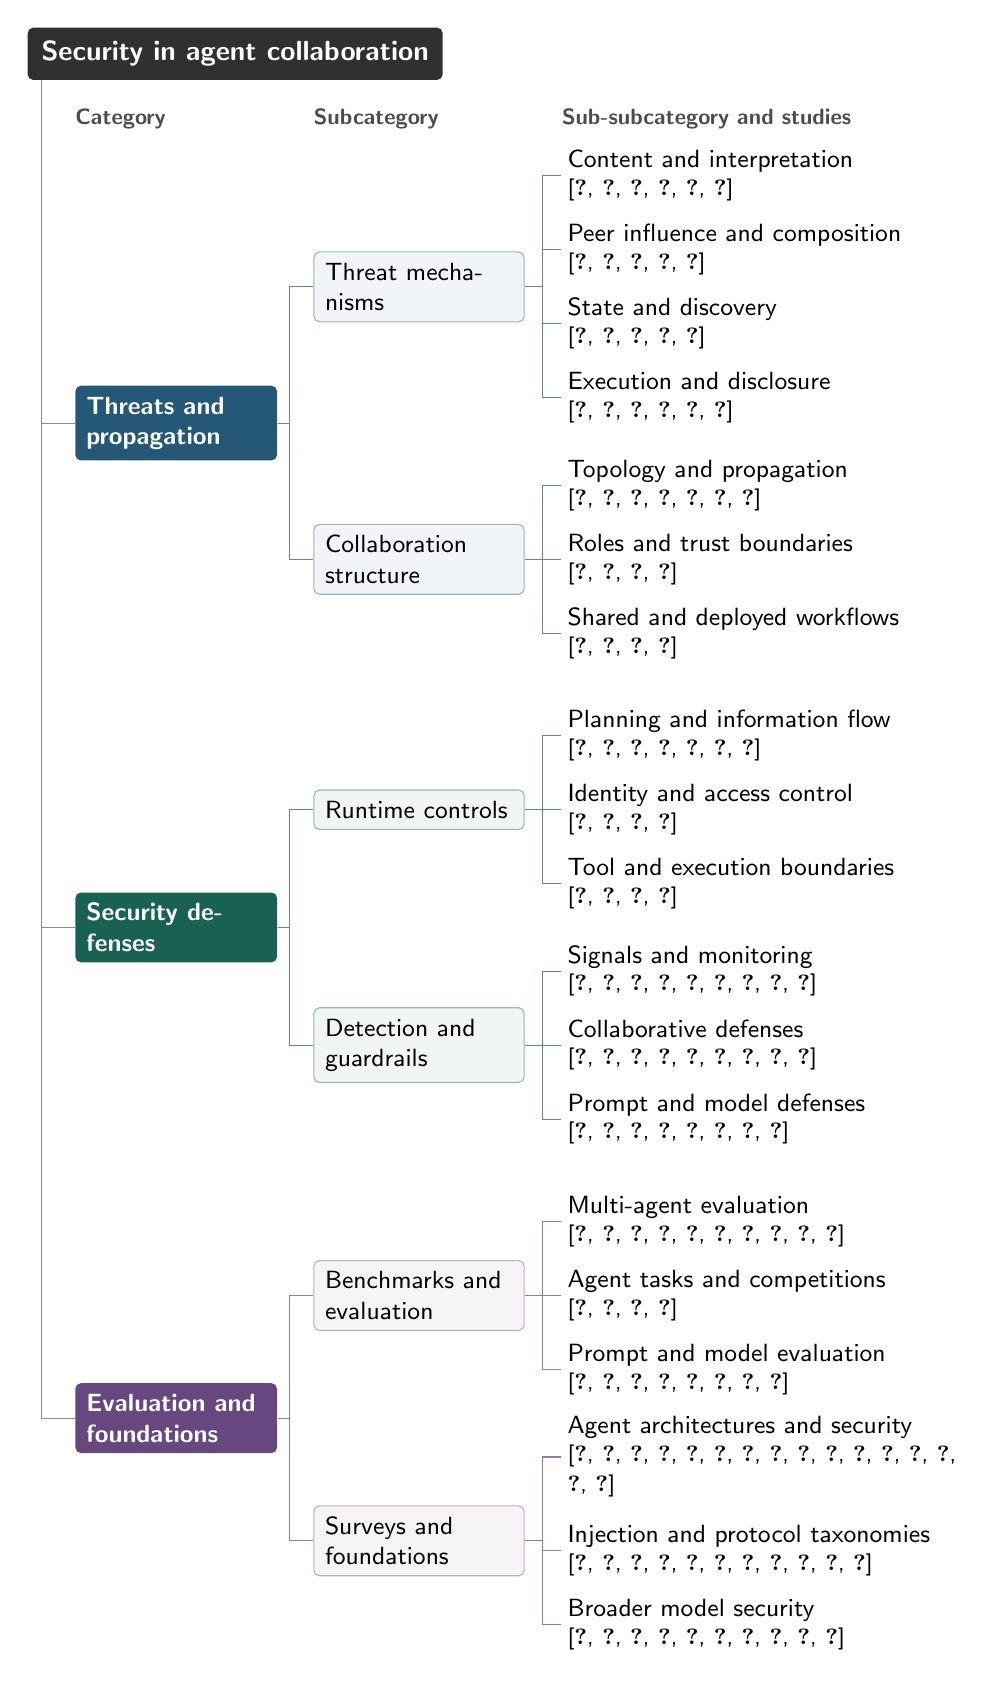
\begin{tikzpicture}[x=.01\linewidth,y=1cm,
  root/.style={anchor=west,rounded corners=2pt,fill=black!81,text=white,inner sep=5pt,font=\sffamily\bfseries},
  cat/.style={anchor=west,align=left,text width=.188\linewidth,inner sep=4pt,rounded corners=2pt,font=\sffamily\small\bfseries},
  sub/.style={anchor=west,align=left,text width=.197\linewidth,inner sep=4pt,rounded corners=2pt,font=\sffamily\small},
  leaf/.style={anchor=west,align=left,text width=.423\linewidth,inner sep=2pt,font=\sffamily\small},
  level/.style={anchor=west,font=\sffamily\footnotesize\bfseries,text=black!70,inner sep=0pt}]
\node[root] (root) at (0,1.42) {Security in agent collaboration};
\node[level] at (5,.59) {Category};
\node[level] at (30,.59) {Subcategory};
\node[level] at (56,.59) {Sub-subcategory and studies};
\definecolor{tier0}{HTML}{245876}
\definecolor{tier1}{HTML}{196253}
\definecolor{tier2}{HTML}{674780}
\coordinate (origin) at (1.5,.98);
\node[leaf] (leaf0) at (56,-0.130) {Content and interpretation\\[-1pt]{\footnotesize\cite{Gu2024AgentSAAO,Sehwag2026ASPISAAH,Yeo2025MultimodalPIBL,Pasquini2024NeuralELAL,greshake2023indirect,Wen2025RLIAU}}};
\node[leaf] (leaf1) at (56,-1.070) {Peer influence and composition\\[-1pt]{\footnotesize\cite{shahroz2025siege,Yan2025AttackTMAQ,arif2026conjunctive,lee2024promptinfection,he2025aitm}}};
\node[leaf] (leaf2) at (56,-2.010) {State and discovery\\[-1pt]{\footnotesize\cite{Chen2024AgentPoisonRLBS,Patlan2025CrossUserPUAK,Sunil2026MemoryPABF,Yu2026MisleadingTPO,Shi2025PromptIAR}}};
\node[leaf] (leaf3) at (56,-2.950) {Execution and disclosure\\[-1pt]{\footnotesize\cite{Pedro2023FromPIBE,Wang2025IPLAX,triedman2025mas,naik2026omnileak,Nagaraja2026WhenPCBF,Kao2026YouTMAZ}}};
\node[sub,fill=tier0!6,draw=tier0!45] (sub0) at (30,-1.540) {Threat mechanisms};
\coordinate (spine0) at (54,-1.540);
\node[leaf] (leaf4) at (56,-4.060) {Topology and propagation\\[-1pt]{\footnotesize\cite{hagag2026architecture,Hu2026AttackingADAX,Le2026CrosslayerCOAI,Malla2026FromMTI,Xie2026FromSTBA,Zhu2025MASTERMSR,Yu2025NetSafeETBB}}};
\node[leaf] (leaf5) at (56,-5.000) {Roles and trust boundaries\\[-1pt]{\footnotesize\cite{Paul2026BeyondSIE,peigne2025securitytax,Liu2026TheCPT,Mitra2026WhereREC}}};
\node[leaf] (leaf6) at (56,-5.940) {Shared and deployed workflows\\[-1pt]{\footnotesize\cite{Mitra2026AgenticCyOpsSMAH,Jamshidi2026SecurityEOAG,Wang2025ShadowsITAL,Nakamura2025TerrariumRTAR}}};
\node[sub,fill=tier0!6,draw=tier0!45] (sub1) at (30,-5.000) {Collaboration\\structure};
\coordinate (spine1) at (54,-5.000);
\node[cat,fill=tier0,text=white] (cat0) at (5,-3.270) {Threats and\\propagation};
\coordinate (split0) at (27.5,-3.270);
\node[leaf] (leaf7) at (56,-7.240) {Planning and information flow\\[-1pt]{\footnotesize\cite{Mao2025AgentSafeSLY,jha2025controlvalve,debenedetti2025camel,li2025drift,an2025ipiguard,wu2024ifc,Hu2026TwinACI}}};
\node[leaf] (leaf8) at (56,-8.180) {Identity and access control\\[-1pt]{\footnotesize\cite{Tallam2026AuthorizationPIBH,Zou2025BlockA2ATSAC,Narajala2025SecuringGMAU,Ji2026TamingVPAP}}};
\node[leaf] (leaf9) at (56,-9.120) {Tool and execution boundaries\\[-1pt]{\footnotesize\cite{Taheri2020MitigationARBP,Engelmann2022RV4JaCaRBL,Rashidi2026TheBOBQ,Li2026UniversalDFL}}};
\node[sub,fill=tier1!6,draw=tier1!45] (sub2) at (30,-8.180) {Runtime controls};
\coordinate (spine2) at (54,-8.180);
\node[leaf] (leaf10) at (56,-10.230) {Signals and monitoring\\[-1pt]{\footnotesize\cite{Malik2026ADLK,Cai2026CrossLayerSFBK,Alamsabi2026EmbeddingBasedDOX,Li2026MESAPVAS,Hashmi2026PromptIDBR,Shi2026SAIGuardCSN,Gosmar2025SentinelAFAJ,Xu2026WhenAGQ,Xie2025WhosTMAI}}};
\node[leaf] (leaf11) at (56,-11.170) {Collaborative defenses\\[-1pt]{\footnotesize\cite{Hossain2025AMLV,Miao2025BlindGuardSLAV,Luo2026DefendingLMV,Wang2025GSafeguardATAW,Kachuee2026MASGuardUGW,Wang2025MASShieldADAF,Zhang2026OpenEvoShieldDNZ,Gosmar2025PromptIDY,Yan2026PropGuardSLAE}}};
\node[leaf] (leaf12) at (56,-12.110) {Prompt and model defenses\\[-1pt]{\footnotesize\cite{Shaheer2025BeyondTBAW,Chen2024DefenseAPBG,Li2024InjecGuardBABC,Piet2023JatmoPIAS,li2025piguard,Gosmar2026PromptIMAA,Ramakrishnan2025SecuringAAAA,chen2025struq}}};
\node[sub,fill=tier1!6,draw=tier1!45] (sub3) at (30,-11.170) {Detection and guardrails};
\coordinate (spine3) at (54,-11.170);
\node[cat,fill=tier1,text=white] (cat1) at (5,-9.675) {Security defenses};
\coordinate (split1) at (27.5,-9.675);
\node[leaf] (leaf13) at (56,-13.410) {Multi-agent evaluation\\[-1pt]{\footnotesize\cite{An2026ACIArenaTUH,Ogunjinmi2026AgenticARN,Carolina2025EvaluatingMDAX,MateoTorrejon2026GAMMAFACAG,Liu2026MADBenchBTU,Hagag2026ORBITAFAD,Zhang2024PsySafeACAN,kavathekar2025tamas,Sharma2025TowardsUQBD,Wang2026TrinityGuardAUF}}};
\node[leaf] (leaf14) at (56,-14.350) {Agent tasks and competitions\\[-1pt]{\footnotesize\cite{zhang2025asb,Dziemian2026HowVAAN,zhan2024injecagent,Zou2025SecurityCIAD}}};
\node[leaf] (leaf15) at (56,-15.290) {Prompt and model evaluation\\[-1pt]{\footnotesize\cite{Yi2023BenchmarkingADAR,Wan2024CYBERSECEVAL3ABJ,liu2024formalizing,Li2024GenTelSafeAUAU,Liu2026LongPIBenchALAV,aal2025PromptIABT,Benjamin2024SystematicallyAPBK,Toyer2023TensorTIAM}}};
\node[sub,fill=tier2!6,draw=tier2!45] (sub4) at (30,-14.350) {Benchmarks and\\evaluation};
\coordinate (spine4) at (54,-14.350);
\node[leaf] (leaf16) at (56,-16.400) {Agent architectures and security\\[-1pt]{\footnotesize\cite{Shahriar2025ASOE,Yu2025ASOL,Siu2026AgentSNZ,Xiang2026ArchitectingSAAP,Zhu2026BlockchainETAT,Luo2025LargeLMBI,Hossain2026OnUIS,Witt2025OpenCIBE,Rafe2026OrchestrationAVK,Xu2026SecurityAAJ,Wang2025SecurityOIBN,Owoputi2022SecurityOMD,Yang2026SoKWSJ,RahulDevT2026TowardSAG,Ling2026TowardSLG,Li2026TowardsSABM}}};
\node[leaf] (leaf17) at (56,-17.590) {Injection and protocol taxonomies\\[-1pt]{\footnotesize\cite{Cao2026ASSM,Yadav2025AdversialPIBA,Song2025BeyondTPAE,Mao2025FromLTAY,Ferrag2025FromPIB,McHugh2025PromptI2F,Prabhakarn2026PromptIAAZ,Geng2025PromptIABB,Mourad2026SecuringTPAQ,Rababah2024SoKPHBH,Wang2026TheLOT}}};
\node[leaf] (leaf18) at (56,-18.530) {Broader model security\\[-1pt]{\footnotesize\cite{Xu2025ASOAT,Chowdhury2024BreakingDTBQ,Liu2024ExploringVABS,Ferrag2024GenerativeAIBM,Peng2024JailbreakingAMAY,S2025ModernDLAC,Cui2024RecentAIBO,Peng2024SecuringLLBR,Das2024SecurityAPBP,Li2025SecurityCFBN}}};
\node[sub,fill=tier2!6,draw=tier2!45] (sub5) at (30,-17.465) {Surveys and\\foundations};
\coordinate (spine5) at (54,-17.465);
\node[cat,fill=tier2,text=white] (cat2) at (5,-15.907) {Evaluation and foundations};
\coordinate (split2) at (27.5,-15.907);
\draw[tier0!72] (spine0) |- (leaf0.west);
\draw[tier0!72] (spine0) |- (leaf1.west);
\draw[tier0!72] (spine0) |- (leaf2.west);
\draw[tier0!72] (spine0) |- (leaf3.west);
\draw[tier0!72] (sub0.east)--(spine0);
\draw[tier0!72] (split0) |- (sub0.west);
\draw[tier0!72] (spine1) |- (leaf4.west);
\draw[tier0!72] (spine1) |- (leaf5.west);
\draw[tier0!72] (spine1) |- (leaf6.west);
\draw[tier0!72] (sub1.east)--(spine1);
\draw[tier0!72] (split0) |- (sub1.west);
\draw[tier0!72] (cat0.east)--(split0);
\draw[black!45] (origin) |- (cat0.west);
\draw[tier1!72] (spine2) |- (leaf7.west);
\draw[tier1!72] (spine2) |- (leaf8.west);
\draw[tier1!72] (spine2) |- (leaf9.west);
\draw[tier1!72] (sub2.east)--(spine2);
\draw[tier1!72] (split1) |- (sub2.west);
\draw[tier1!72] (spine3) |- (leaf10.west);
\draw[tier1!72] (spine3) |- (leaf11.west);
\draw[tier1!72] (spine3) |- (leaf12.west);
\draw[tier1!72] (sub3.east)--(spine3);
\draw[tier1!72] (split1) |- (sub3.west);
\draw[tier1!72] (cat1.east)--(split1);
\draw[black!45] (origin) |- (cat1.west);
\draw[tier2!72] (spine4) |- (leaf13.west);
\draw[tier2!72] (spine4) |- (leaf14.west);
\draw[tier2!72] (spine4) |- (leaf15.west);
\draw[tier2!72] (sub4.east)--(spine4);
\draw[tier2!72] (split2) |- (sub4.west);
\draw[tier2!72] (spine5) |- (leaf16.west);
\draw[tier2!72] (spine5) |- (leaf17.west);
\draw[tier2!72] (spine5) |- (leaf18.west);
\draw[tier2!72] (sub5.east)--(spine5);
\draw[tier2!72] (split2) |- (sub5.west);
\draw[tier2!72] (cat2.east)--(split2);
\draw[black!45] (origin) |- (cat2.west);
\draw[black!45] (origin |- root.south) -- (origin);
\end{tikzpicture}
\caption{Taxonomy of 137 studies by primary research focus. Each path connects a category to a subcategory and then to a cited sub-subcategory.}\label{fig:inert-corpus-tree}
\end{figure}
\clearpage
\ifdefined\INERTmanuscript\else
\bibliographystyle{plainnat}
\bibliography{injection_channel_taxonomy}
\fi
\ifdefined\INERTmanuscript\else\expandafter\enddocument\fi
